% resDoc.tex

\documentclass[11pt]{book}
\usepackage{resDocSty}         % Res Doc .sty file
\usepackage{appendix}
\usepackage{cite}

\usepackage{longtable,array}   % need array when specifying a ragged right column:  >{\raggedright\arraybackslash}{p2in}.
% \renewcommand{\chaptername}{Appendix}
% \renewcommand*{\chaptername}{Appendix}
% \addto\captionsenglish{\renewcommand\chaptername{Part}}
\usepackage{import}            % for figures in chapter subdirectories

% Had these for YMR Eqns appendix:
% \renewcommand{\footrulewidth}{0.4pt}
% \renewcommand{\headrulewidth}{0pt}

% For appendices:
\usepackage{graphicx}          % For inclusion of figures
\usepackage{verbatim,fancyvrb} % Check - may be in .sty file
\usepackage{xifthen}           % provides \ifthenelse and \isempty
\usepackage{color, colortbl}
\usepackage{arydshln}          % For dashed lines in tables (has to be loaded after other stuff)

% For hyperlinked references (figures and citations, etc.). The bookmarksdepthlevel allows
%  the TOC to be shown in the bookmarks tree in the output PDF.
\usepackage[bookmarks,bookmarksopen,bookmarksdepth=4]{hyperref}
\hypersetup{                   % Set up the hyperref options here
    pdftitle={Arrowtooth Flounder},
    pdfauthor={Chris Grandin},
    pdfsubject={Stock Assessment},
    %pdfkeywords={keyword1, keyword2},
    bookmarksnumbered=true,
    bookmarksopen=true,
    bookmarksopenlevel=1,
    colorlinks=true,
    allcolors=blue,
    citecolor=cyan,
    pdfstartview=Fit,
    pdfpagemode=UseOutlines
    %pdfpagelayout=TwoPageRight
}
% Use the following codes for references within the document.
%   chap: chapter
%    sec: section
% subsec: subsection
%    fig: figure
%    tab: table
%     eq: equation
%    lst: code listing
%    itm: enumerated list item
%    app: appendix subsection
\usepackage{hypcap}            % So links will anchor at figure, not caption

\usepackage{subfig}            % For two-panel plots
\usepackage{scrextend}         % For indenting blocks of text with 'addmargin'
\usepackage{relsize}           % For mathlarger, which makes equations bigger
\usepackage{enumitem}          % To remove spacing between list items [noitemsep,nolistsep]
%\usepackage{mathtools}         % For mathmboxes for use in the equations appendix

\definecolor{rowclr}{RGB}{255, 192, 203}
\newcommand{\sQuote}[1]{`#1'}
\newcommand{\dQuote}[1]{``#1''}
\newcommand{\eqn}[1]{\begin{equation}#1\end{equation}}
\newcommand{\gfrac}[2]{\genfrac{}{}{}{0}{#1}{#2}}

\newcommand\bestfig[6]{ % #1=filename, #2=main caption, #3=figure height, #4=short caption #5=file extension #6=directory
	% needs package epstopdf to work
	\begin{figure}[htpb] %[htbp]
	\centering
	\ifthenelse{ \isempty{#5} \OR \equal{#5}{eps} }
		{\includegraphics[width=6.5in,height=#3in,keepaspectratio=TRUE]{#6#1.eps}}
		{\setlength\fboxsep{0pt}
		 \setlength\fboxrule{0pt}
		 \fbox{\includegraphics[width=6.5in,height=#3in,keepaspectratio=TRUE]{#6#1.#5}}}
	% source: http://xelatex.blogspot.ca/2008/03/newcommand-with-optional-argument.html
	\ifthenelse{\isempty{#4}}
		{\caption[#2]{#2}}  % \vspace{-2ex}} AME removing
		{\caption[#4]{#2}}  % \vspace{-2ex}}  ``
	\label{fig:#1}
	\end{figure}
        }

\newcommand\pbsfig[5]{    % #1=filename, #2=main caption, #3=figure height, #4=short caption, #5=directory
	\begin{figure}[tp] %[htbp]  Rowan had ht!
	\centering
	\includegraphics[width=6.5in,height=#3in,keepaspectratio=TRUE]{#5#1.eps}
	% source: http://xelatex.blogspot.ca/2008/03/newcommand-with-optional-argument.html
	\ifthenelse{\isempty{#4}}
		{\caption[#2]{#2}\vspace{-2ex}}
		{\caption[#4]{#2}\vspace{-2ex}}
	\label{fig:#1}
	\end{figure}
	%\clearpage
}

% eor - Show two things with a vertical bar between them
\newcommand{\eor}[2]{{#1$\Vert$#2}}
% bM - makes equations larger
\newcommand{\bM}[1]{\mathlarger{\mathlarger{#1}}}
% Allow newline breaks in a table cell: syntax is \specialcell{first line\\secondline}
\newcommand{\specialcell}[2][c]{\begin{tabular}[#1]{@{}c@{}}#2\end{tabular}}

\newcommand{\fishname}{Arrowtooth Flounder}
% sciencename - Science name for the species being assessed
\newcommand{\sciencename}{Atheresthes stomias}

% Headers and footers
% For Res Doc, best to have a left and a right footer
%  (and/or header), not just one (for double-sided printing).
%
% \lhead{DRAFT -- Non-citable working paper}  % Omit for final ResDoc.
\lhead{}
\rhead{}
\lfoot{\fishname}           % Species common name for left footer
\rfoot{Coastwide}           % The area of the assessment for right footer
%\rfoot{WP 2012/P02a}       % Change to appendix number for appendices
                            % Will probably delete footers in main text
                            %  for final Res Doc.

% \linenumbers              % uncomment to add in line numbers
% \modulolinenumbers[5]     % just number every 5th line

% \def\AppLet{F}            % Appendix letter - we had this
                            %  to number equations in Appendix
                            %  F as (F.17) etc.
% \def\StartP{102}          % page start

\newcommand{\Bmsy}{B_\mathrm{MSY}}
\newcommand{\umsy}{u_\mathrm{MSY}}
\newcommand{\MapData}{C:/Work/ArrowtoothFlounder/2014Assessment/data/MapData}

\newcommand{\EstM}{`Estimate \emph{M}'}
\newcommand{\FixM}{`Fix \emph{M}'}

\begin{document}


% preamble.tex - Tables of Contents, Figures, Tables, plus Abstract
%  Useful to comment out when don't need all that (e.g. working on an
%  Appendix).

%%CoverPage
%\input{./csasCoverPage} - currently using word->pdf and merging pdfs
%  for ResDocs.
%\newpage
% For working paper, use this before using Word for actual submission.

% From Matt Grinnel's Tech Report document.
%\setlength{\parindent}{0mm}
\thispagestyle{fancyplain}
%\pagecolor{Tan}

\pagenumbering{roman}

\begin{flushleft}
\LARGE \textbf{Arrowtooth Flounder ({\bf \emph{Atheresthes stomias}}) stock assessment for the west coast of British Columbia}

% \TRtitleCap}
\end{flushleft}
\vfill
{\Large Chris Grandin, Robyn Forrest, and Paul J. Starr}
\vfill
% \TRaddy
\vfill
% \TRyear
\vfill
{\LARGE \textbf{Working paper number 2014/ARF01}}\\
 % Canadian Technical Report of\\Fisheries and Aquatic Sciences  \TRreportNumber}
\vspace{2cm}
[Replace with Word template for submission]
\vfill
% \lfoot{\includegraphics[height=5mm]{doc/DFOleft.jpeg}}
% \cfoot{}
% \rfoot{\includegraphics[height=5mm]{doc/DFOright.png}}
\clearpage

%% ---------------------------------------------------------------------

%%TOC will go here (page iii - req'mt by CSAS)
% \setcounter{page}{3}
\renewcommand{\contentsname}{\bf \large \vspace{-25mm} TABLE OF CONTENTS}
\addtocontents{toc}{\protect\thispagestyle{fancy}}
% \renewcommand{\cftchapterfont}{APPENDIX }\setlength{\cftfignumwidth}{1.5em}     % - ask Jaclyn, want to make it same as others.
%\begin{center}
%\tableofcontents
%\end{center}
%\newpage

% \nonumsection*{TABLE OF CONTENTS}

\begin{center}
\tableofcontents
\end{center}
\newpage

% Use Word template for these and cover page (use final YMR).

% Andy not using:
% \addtocontents{lof}{\protect\thispagestyle{fancy}}
%\renewcommand{\listfigurename}{\bf \large \vspace{-25mm} LIST OF MAIN FIGURES}     % JC and AME decided to restrict to just main ones.
%\renewcommand{\cftfigfont}{Figure }\setlength{\cftfignumwidth}{1.5em}
%\begin{center}
%\listoffigures
%\end{center}
%\addcontentsline{toc}{section}{LIST OF MAIN FIGURES}
%\newpage

%\addtocontents{lot}{\protect\thispagestyle{fancy}}
%\renewcommand{\listtablename}{\bf \large \vspace{-25mm} LIST OF MAIN TABLES}
%\renewcommand{\cfttabfont}{Table }\setlength{\cfttabnumwidth}{1.5em}
%\begin{center}
%\listoftables
%\end{center}
%\addcontentsline{toc}{section}{LIST OF MAIN TABLES}
%\clearpage

\leftskip=3em	%%required to indent Citation below
\parindent=-3em

{\bf Correct citation for this publication:}

Non-citable Working Paper.	%%(req'mt by CSAS)

%Cleary, J.S. and Haist, V. 2012.****
%Stock Assessment and Management Advice for the British Columbia Pacific Herring Stocks: 2012 Assessment and 2013 Forecasts.
%DFO Can. Sci. Advis. Sec. Res. Doc. 2012/xxx. xii + 151 p.

%JSC: would be nice to automate roman and regular page numbers. Counter? See Matt Grinnell's Tech Report latex files.

\leftskip=0em	%% end Citation indent
\parindent=-0em

%% \section*{Abstract}\addcontentsline{toc}{section}{ABSTRACT}
%% \nonumsection is centered
%\nonumsection*{ABSTRACT}\addcontentsline{toc}{section}{ABSTRACT}

% \newpage	%French abstract must appear on new page

%% \section*{R\'esum\'e}\addcontentsline{toc}{section}{R\'ESUM\'E}
% \nonumsection*{R\'ESUM\'E}\addcontentsline{toc}{section}{R\'ESUM\'E}

% \addcontentsline{toc}{section}{R\'ESUM\'E}

% hareng de la C.-B. sont g\'er\'es en fonction de cinq zones de stocks principales et de deux zones secondaires. En cons\'equence, l'information sur les prises et celle provenant des relev\'es est recueillie de fa\c{c}on ind\'ependante pour les sept zones, et on formule des avis scientifiques pour chacune. On s'est servi de toutes les donn\'ees biologiques disponibles sur la ponte, la composition selon l'\^{a}ge et la taille des stocks reproducteurs ainsi que sur les pr\'el\`{e}vements de la p\^{e}che commerciale pour d\'eterminer les niveaux d'abondance actuels. Ces derni\`{e}res ann\'ees, des examinateurs externes ont sugg\'er\'e que d'importantes r\'evisions soient apport\'ees au cadre d'\'evaluation du hareng, y compris au mod\`{e}le des prises selon l'\^{a}ge. Nous pr\'esentons donc un nouveau mod�le statistique int\'egr\'e des prises selon l'\^{a}ge (iSCAM) pour estimer conjointement l'abondance des stocks de hareng du Pacifique et les points de r\'ef\'erence connexes (partie I). Ce mod\`{e}le comprend des essais de simulation pour d\'emontrer que le mod\`ele peut estimer tous les param\`{e}tres ainsi qu'une param\'etrisation du nouveau mod\`{e}le d�\'evaluation comme le pr\'ec\'edent mod\`{e}le d�\'evaluation (mod\`{e}le des prises de hareng selon l'\^{a}ge ou HCAM) pour que l�on puisse comparer les estimations des param\`{e}tres et les estimations de la biomasse du stock reproducteur (en utilisant les donn\'ees de 1951 \`{a}) 2010) entre l'ancien mod\`{e}le (HCAM) et le nouveau (ISCAM). La partie II de ce document refl\`{e}te le nouveau cadre d'\'evaluation avec des donn\'ees des cinq zones de stock principales et des deux zones secondaires. Finalement, nous pr\'esentons des estimations de la biomasse avant la p\^{e}che et un avis sur les prises fond\'e sur les tableaux sur les d\'ecisions qui utilisent les pr\'evisions du recrutement \`{a} l'\^{a}ge 3 faible, moyen et bon ainsi que sur les tableaux sur la probabilit\'e du risque afin d'\'eclairer la prise de d\'ecision.



              % Table of contents, etc.
% \setcounter{chapter}{0}
% \setcounter{table}{0}
% \setcounter{figure}{0}
\setcounter{secnumdepth}{3}    % To number subsubheadings-ish

% To number sections, tables etc. as 1, 2, 3, not 1.1 etc. (where
%  the first 1 would be chapter number).
\renewcommand{\thesection}{\arabic{section}}
\renewcommand{\thetable}{\arabic{table}}
\renewcommand{\thefigure}{\arabic{figure}}
\renewcommand{\theequation}{\arabic{equation}}

% \subimport{mainDoc/}{mainDocRev}
\input{maindoc/maindoc}

\clearpage

% \addcontentsline{toc}{chapter}{Appendices}
\addtocontents{toc}{\par {\bf \vspace{10mm} APPENDICES} \par}
\addtocontents{toc}{\protect\setcounter{tocdepth}{0}}
\appendix           % Everything from now on will be an Appendix
% \begin{appendices}

% \renewcommand{\appendixname}{Appendix} - doesn't work
% \renewcommand*{\chaptername}{Appendix} - never worked
% Also tried in .sty file.

% Now want to number sections, tables etc. as A.1, A.2, etc.
% Thought these wouldn't be with the appendix package, as
%  automatic, but do need them even if use \begin{appendices}:
\renewcommand{\thesection}{\thechapter.\arabic{section}}
\renewcommand{\thetable}{\thechapter.\arabic{table}}
\renewcommand{\thefigure}{\thechapter.\arabic{figure}}
\renewcommand{\theequation}{\thechapter.\arabic{equation}}

% Not including Appendix figures and tables in contents, and just
%  including the Appendix (chapter) names (not sections or
%  subsections):
% Wait for Jaclyn to say how.
% Also to have Appendix title as   Appendix A   not just A. Tried
%  the above but no luck. May have to use the appendix package, and
%  understand better the options. Think it may be getting overridden
%  by the \renewcommand{\chapter}{\@startsection    in resDocSty.sty

\lfoot{Arrowtooth Flounder - Coastwide}

\rfoot{Appendix A -- Biological Data}
% app-biology.tex

\clearpage

\chapter{BIOLOGICAL DATA}

These analyses have been performed on a GFBio extract dated 18 August 2014. We used the following data selection criteria for all the following analyses (the [agemeth] and [maturity] criteria were only used when the analyses required these data):

\section{Length and Weight Analyses}

After extracting all valid length/weight pairs of data based on the criteria shown in table~\ref{tab:bioCrit}, we used the following length-weight equation:

\begin{align} \label{eq:lw}
ln(W_i^s) = b^sln(L_i^s) + a^s + \varepsilon
\end{align}
\begin{addmargin}[3em]{1em}
where $a^s$ and $b^s$ are parameters for sex $s$ and $L_i^s$ and $W_i^s$ are paired length-weight observations.
\end{addmargin}

We only applied Equation~\eqref{eq:lw} to research or charter observations (trip\_type==2 or trip\_type==3) from PMFC areas 3CD5ABCDE. There were some bad data in the lower end of the distribution which possibly biased the analysis (Figure~\ref{fig:lwOptionA}). There are a number of ways to drop these data, including discarding large residuals (Option B: Table~\ref{tab:lwEst}, Figure~\ref{fig:lwOptionB}) or truncating the empirical distribution (We discarded the top and bottom 0.5\% of the distribution: Option C, Table~\ref{tab:lwEst}, Figure~\ref{fig:lwOptionC}). Finally, we combined the two truncation methods as Option D (Table~\ref{tab:lwEst}, Figure~\ref{fig:lwOptionD}). The models resulting from these three truncated analyses all appear to be effectively the same (see Figure~\ref{fig:lwCompare}) and the model using all the data is slightly to the right of the other three for both males and females. The parameter estimates for all four analyses were similar, although the exponent parameter is slightly lower for males and females for Option A (Table~\ref{tab:lwEst}). Option D had the best residual patterns (see Figure~\ref{fig:lwOptionD}) but all three truncated models will have the same impact when included in a biomass population model (Figure~\ref{fig:lwCompare}).  The model provided in Table 2 of \citet{arf2001} is similar to Option A for females but is to the left from the other four options for males (Figure~\ref{fig:lwCompare}).

\section{von-Bertalanffy Analyses}

We used the von-Bertalanffy function to estimate growth rates for \fishname:

\begin{align} \label{eq:vonb}
L_i^s = L_\infty^se^{(-k^s[a_i^s-t_0^s])}
\end{align}
\begin{addmargin}[3em]{1em}
where $L_\infty^s$, $k^s$, and $t_0^s$ are parameters specific to sex $s$ and $L_i^s$ and $a_i^s$ are paired length-age observations.
\end{addmargin}

There are several hundred paired length-age observations in most of the PMFC regions, except for 5A and 5E where the latter has no observations and the former has only a few (Table~\ref{tab:numagesByArea}). PMFC region 5D has about 3,000 age-length pairs which is the result of intensive sampling by the Hecate Strait multi-species assemblage survey. The maximum age of 50 in region 5B is the result of one male observation which was discarded because it was such a large outlier (model parameters were not affected by this single observation when fitted). The distributions by month are concentrated from late spring to mid-summer, with the large majority of the age-length pair originating from May and June (Table~\ref{tab:numagesByArea}). Using these data to estimate an annual growth rate is not ideal, but at least the observations are near mid-season. However, it is possible that this restricted seasonal distribution will lead to an underestimate of the growth rate.

The growth equations were calculated by combining the research and commercial data, and using all months from January to November (Table~\ref{tab:numagesByAreaMonth}). About two-thirds of the observations are from research and charter cruises but the addition of the extra 2,200+ observations from the commercial data has been done to obtain observations from months other than May and June. We calculated growth functions for 3CD as well as one for the combined 5ABCD (there were no 5E observations and relatively few 5A or 5B observations). The preferred model combines all data from the outside PMFC areas (3C to 5D and includes both the research and commercial data) (Figure~\ref{fig:vonb}) in order to obtain observations in months other than May and June. When the three investigated models are superimposed, the differences in estimated growth rates by sex are small, especially for females (Figure~\ref{fig:vonbCompare}). Males and females in 3CD have an  estimate that is \textgreater1 cm larger than for the other two models (Table~\ref{tab:vonbEst}). Males are about 10 cm smaller than females at the same age, which requires that this species should be modelled as with sexes separated (Figure~\ref{fig:vonbCompare}). The female growth function provided by \citet{arf2001} is very similar to the 3CD5ABD function calculated here but the male estimate is about 2-5 cm smaller than the estimates provided in Table~\ref{tab:vonbEst} (Figure~\ref{fig:vonbCompare}).

\section{maturity-at-age Analyses}

Before fitting models to the maturity data, we examined the available female \fishname staging information to ascertain the most likely period during which adult females would be in the reproductive phase (Table~\ref{tab:maturityMonth} and Figure~\ref{fig:maturity}). Given the information in Figure~\ref{fig:maturity}, it seemed most likely that the period over which females were mature extended from at least September to February, with Stage 3 females (Developing in Figure~\ref{fig:maturity}) at their most abundant from July to December and with Stage 4 and Stage 5 females appearing in January and February. The May and June data from the multi-species assemblage survey point to most of the fish being either immature or resting.  The progression of stages seemed consistent between observations generated from the research data and the commercial observers (compare left and right panels in Figure~\ref{fig:maturity}). This consistency between the two sets of observations is important because the amount of research data available to characterise this species is relatively sparse (see Table~\ref{tab:maturityMonth} and Table~\ref{tab:maturityObsPred}), requiring augmenting from the commercial data set.

We used stage 3 (Developing) and higher to define mature females, leaving stages 1 and 2 for immature \fishname. The number of mature females relative to the total number of valid otolith observations at each age was used as the data observation for each age (Equation~\ref{eq:matage1}). These proportions were fitted to a “double-normal” (half-Gaussian) function where the right-hand limb was constrained such that maturity equalled 1.0 when the age was greater than (Equation~\ref{eq:matage2}):

\begin{align} \label{eq:matage1}
P_a^f=N_a^{3-7}/N_a^{1-7}
\end{align}
\begin{addmargin}[3em]{1em}
where $P_a^f$ is the observed proportion mature at age $a_f$ calculated from the sum of valid observations at age for stages 3-7 ($N_a^{3-7}$) divided by the total number of staged females ($N_a^{1-7}$);
\end{addmargin}

\begin{align} \label{eq:matage2}
\hat{P}_a^f=
  \begin{cases}
    e^{\left(-\left(a^f-A^f\right)^2/e^{{\upsilon}L^f}\right)} & \text{if } a^f \leq A^f \\
                                              1 & \text{if } a^f > A^f
  \end{cases}
\end{align}
\begin{addmargin}[3em]{1em}
where $A^f$ and ${\upsilon}L^f$ are parameters for sex $f$ and $\hat{P}_a^f$ is the estimated proportion mature at age $a^f$;
\end{addmargin}

There were only 129 female age observations (of which only 3 were immature) with corresponding maturity data spanning the period July to February (see Table~\ref{tab:maturityObsPred}), leading to an estimated maturity curve that is not credible due to the lack of information at younger ages (Figure~\ref{fig:maturityfit}). More credible maturity ogives are generated with the addition of the May and June data, with little sensitivity to the inclusion or exclusion of the commercial observer data (Figure~\ref{fig:maturityOgiveCompare}). However, this ogive should be used with caution because it may be too spread out because of the difficulty of distinguishing between mature and immature fish at younger ages based on the macroscopic inspection of gonads.

It is not possible to compare this ogive with the one provided by \citet{arf2001} because their Figure 3 is a length-based maturity ogive. This figure would be based on the maturity information from the Hecate Strait Assemblage Survey, but this ogive would be sensitive to the same uncertainty in the maturity determinations as discussed in the previous paragraph.

% FIGURES
\begin{figure}[htp]
\captionsetup[subfigure]{labelformat=empty}
\begin{center}
%\subfloat[]{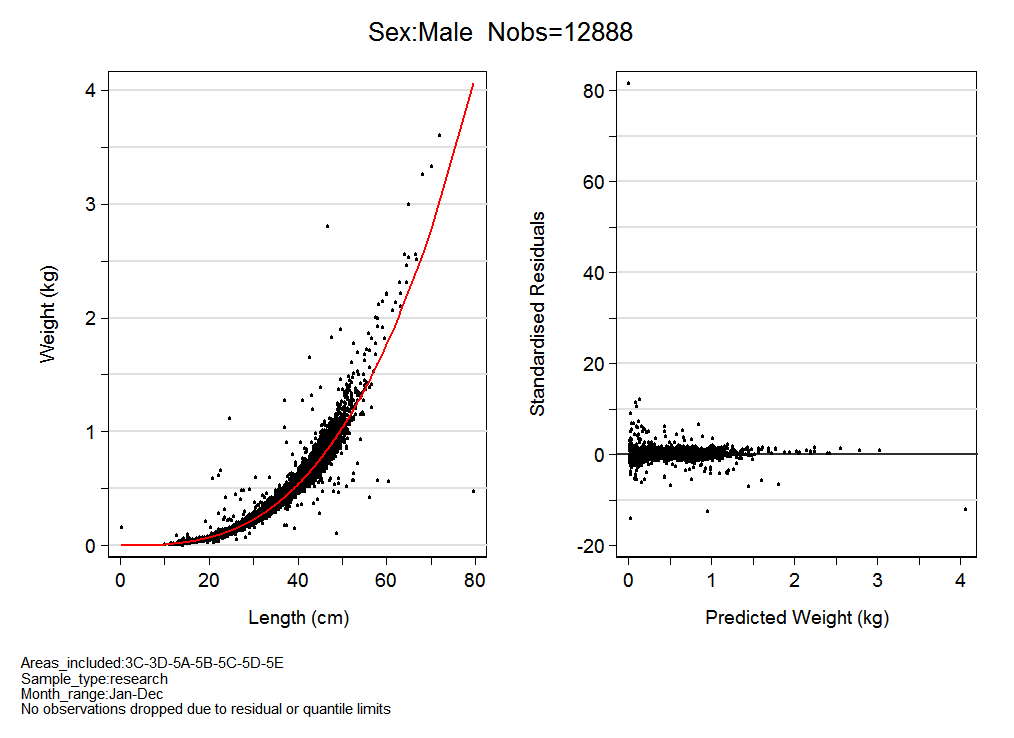
\includegraphics[bb=0 0 925 600,width=6in,keepaspectratio=true]{app-biology/lwmaleOptionA.png}}
\subfloat[]{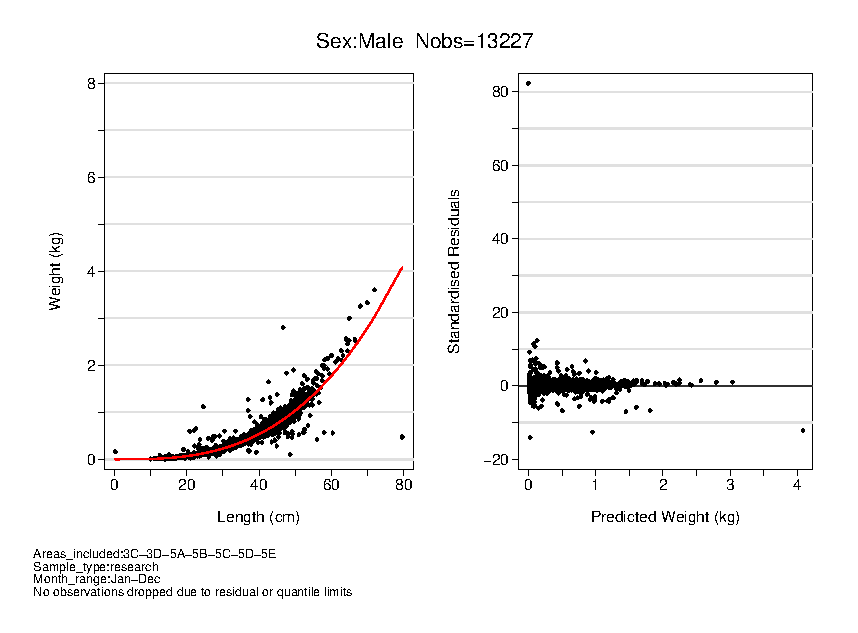
\includegraphics[width=5.7in,keepaspectratio=true]{app-biology/lwmaleOptionA.eps}}
\newline
%\subfloat[]{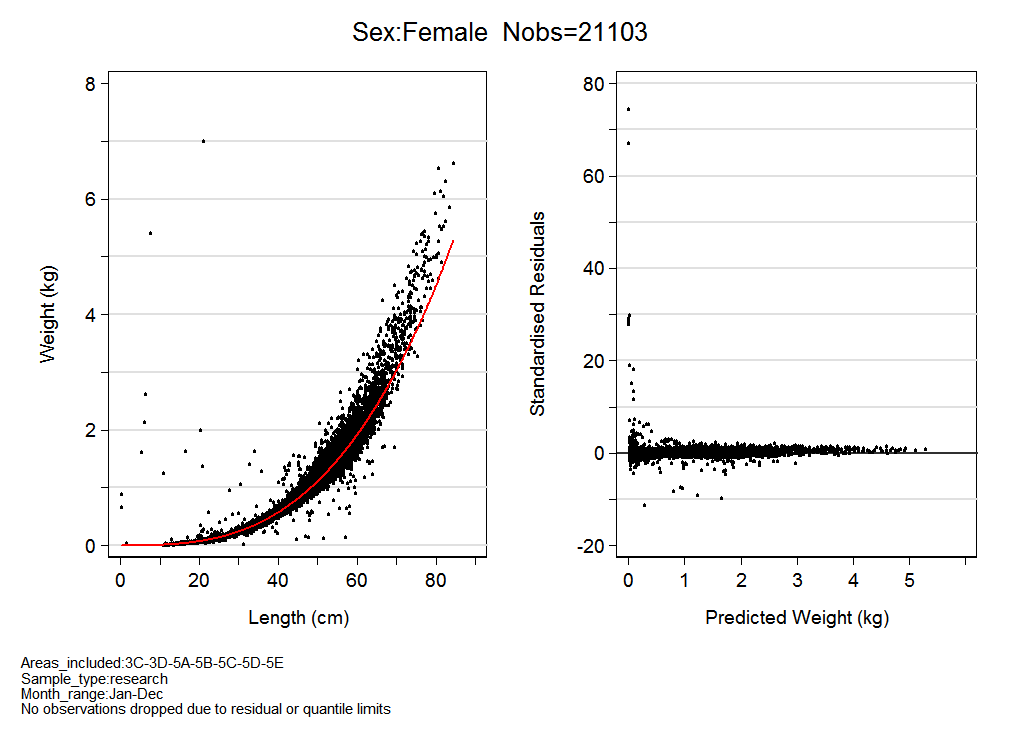
\includegraphics[bb=0 0 925 600,width=6in,keepaspectratio=true]{app-biology/lwfemaleOptionA.png}}
\subfloat[]{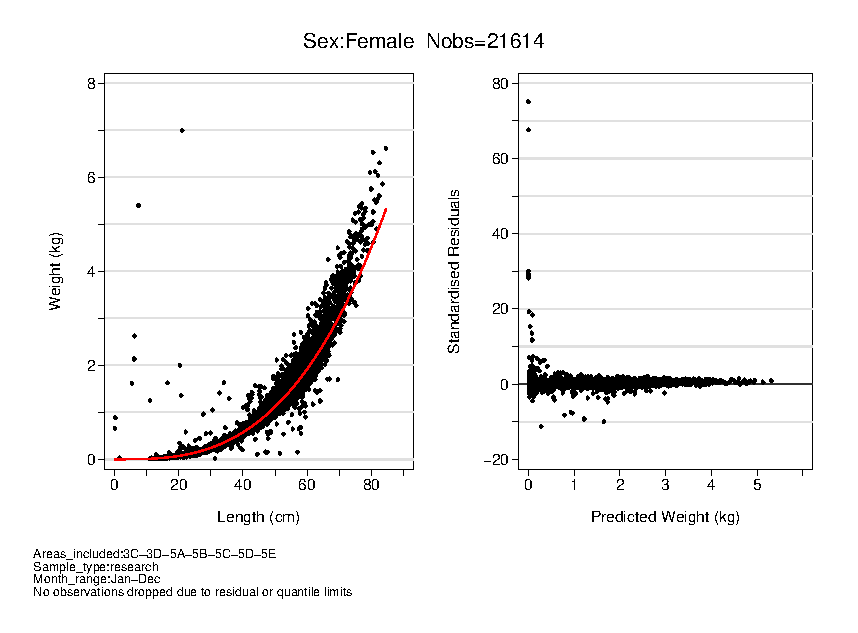
\includegraphics[width=5.7in,keepaspectratio=true]{app-biology/lwfemaleOptionA.eps}}
\end{center}
\vspace{-10mm}
\caption{Length-weight plot for male [top panel] and female [bottom panel] \fishname: combined 3CD5ABCDE with no residual or distributional constraints (option A).}
\label{fig:lwOptionA}
\end{figure}

\begin{figure}[htp]
\captionsetup[subfigure]{labelformat=empty}
\begin{center}
\subfloat[]{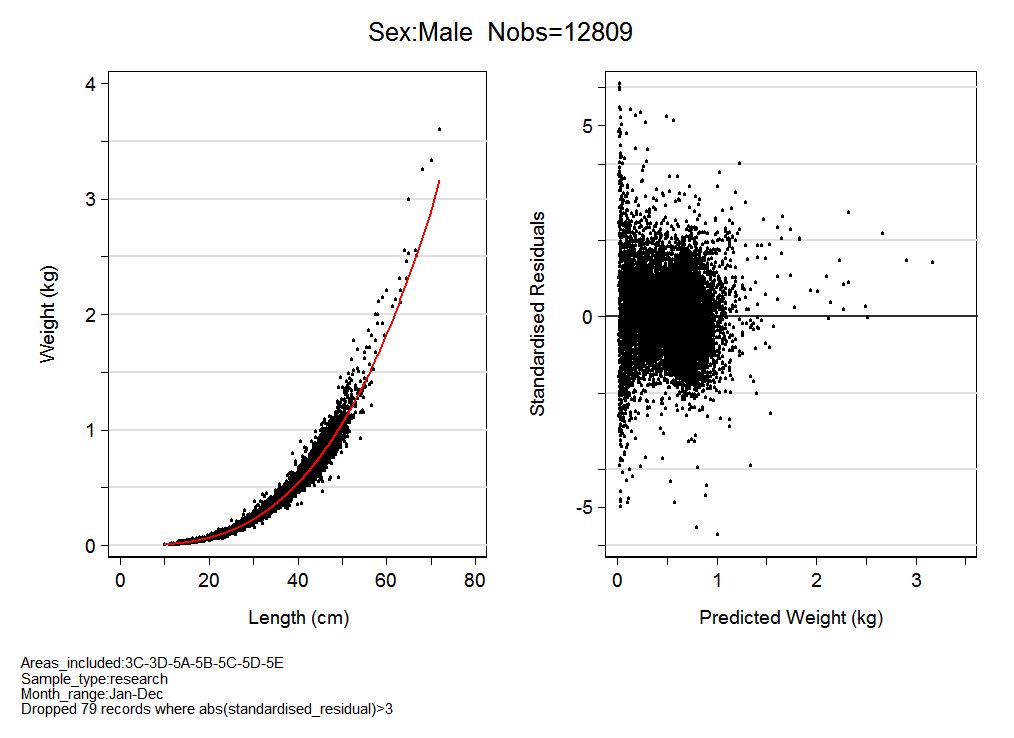
\includegraphics[bb=0 0 925 600,width=6in,keepaspectratio=true]{app-biology/lwmaleOptionB.png}}
\newline
\subfloat[]{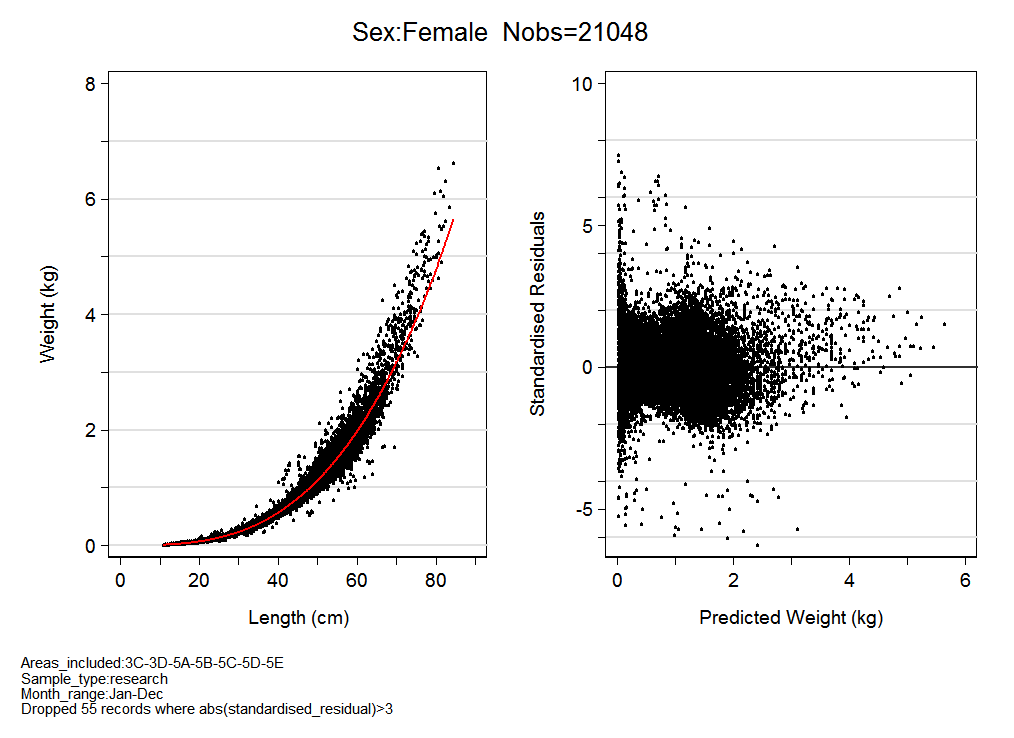
\includegraphics[bb=0 0 925 600,width=6in,keepaspectratio=true]{app-biology/lwfemaleOptionB.png}}
\end{center}
\caption{Length-weight plot for male [top panel] and female [bottom panel] \fishname: combined 3CD5ABCDE with no residual or distributional constraints but discarded standardised residuals (option B).}
\label{fig:lwOptionB}
\end{figure}

\begin{figure}[htp]
\captionsetup[subfigure]{labelformat=empty}
\begin{center}
\subfloat[]{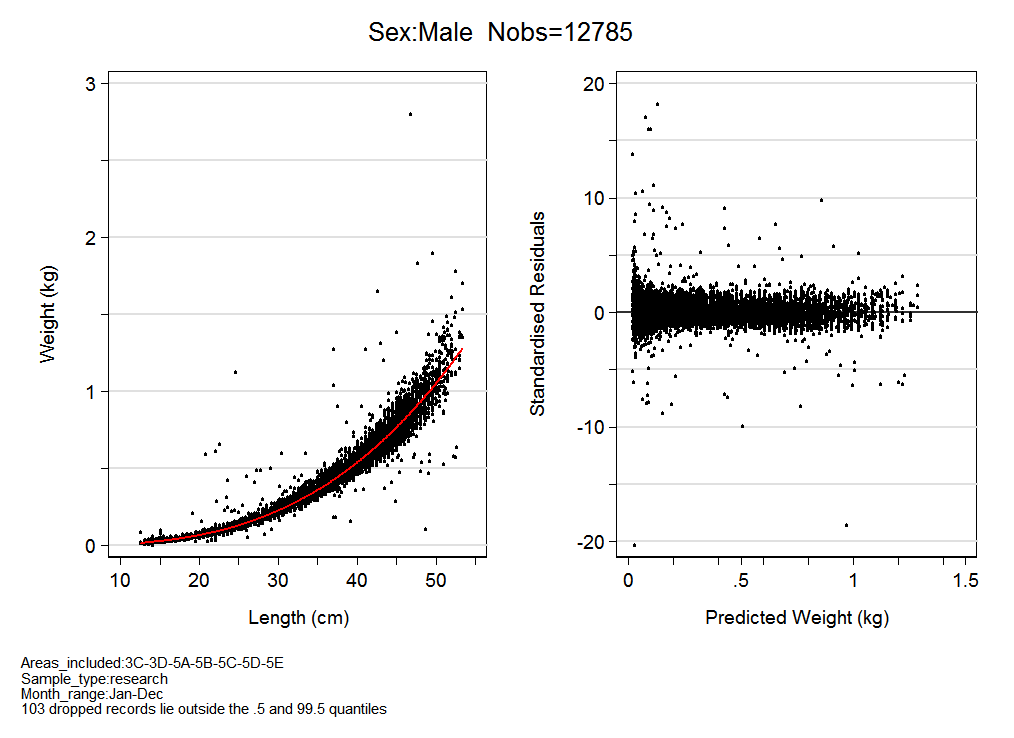
\includegraphics[bb=0 0 925 600,width=6in,keepaspectratio=true]{app-biology/lwmaleOptionC.png}}
\newline
\subfloat[]{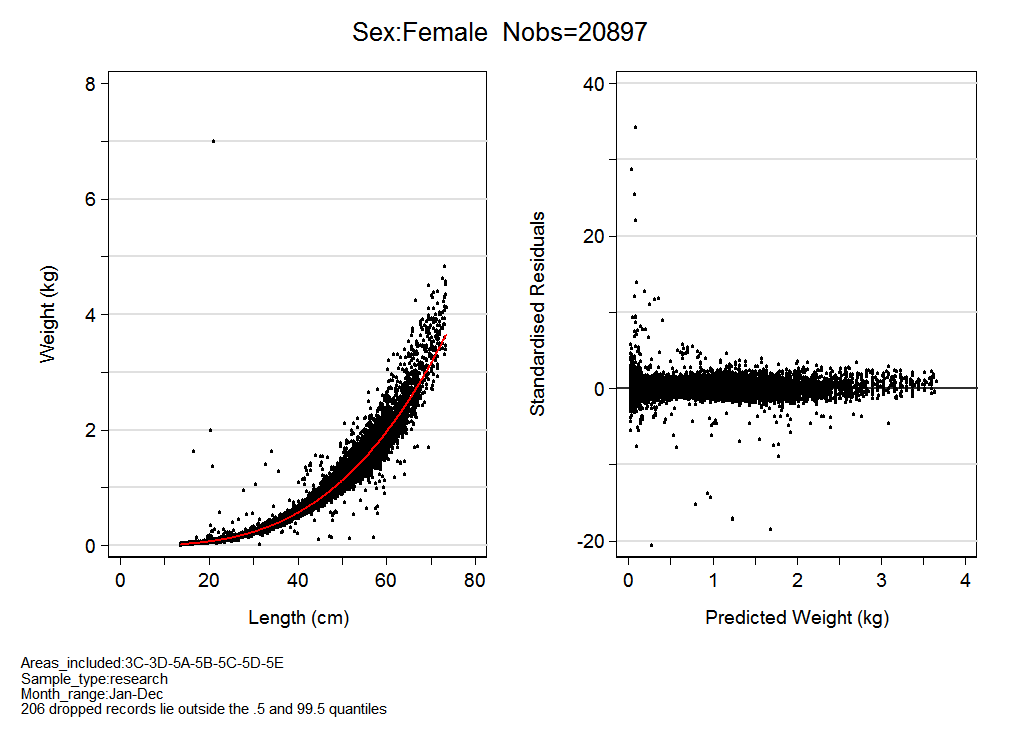
\includegraphics[bb=0 0 925 600,width=6in,keepaspectratio=true]{app-biology/lwfemaleOptionC.png}}
\end{center}
\caption{Length-weight plot for male [top panel] and female [bottom panel] \fishname: combined 3CD5ABCDE with no standardised residuals discarded but with the lower 0.5 and upper 0.95 quantiles of length dropped (option C).}
\label{fig:lwOptionC}
\end{figure}

\begin{figure}[htp]
\captionsetup[subfigure]{labelformat=empty}
\begin{center}
\subfloat[]{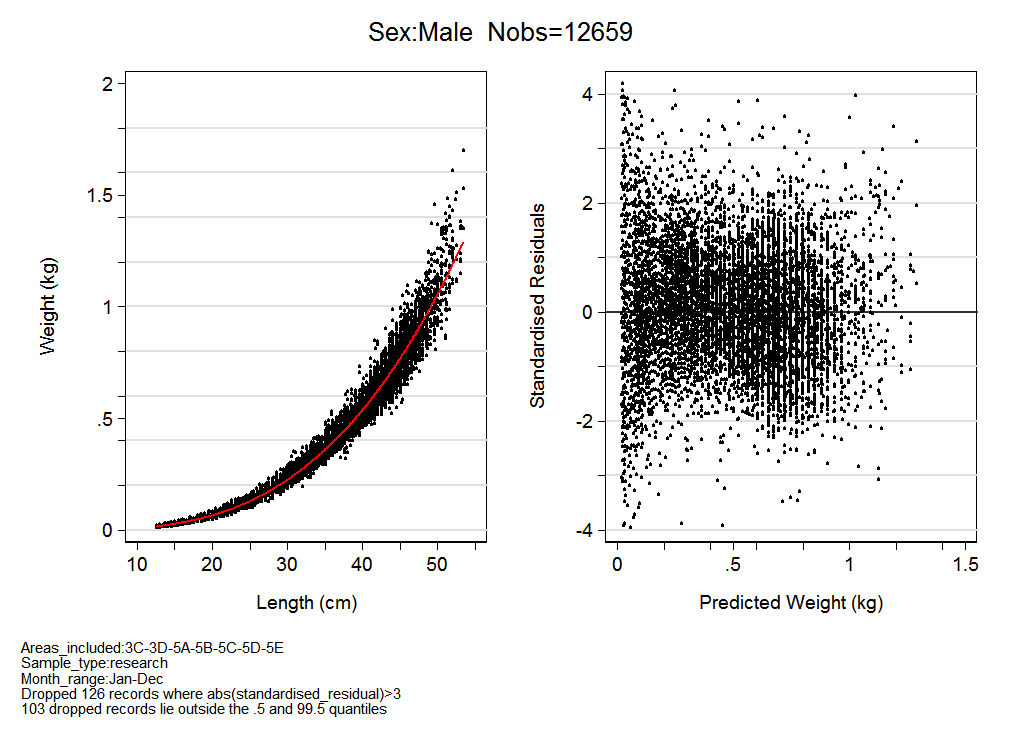
\includegraphics[bb=0 0 925 600,width=6in,keepaspectratio=true]{app-biology/lwmaleOptionD.png}}
\newline
\subfloat[]{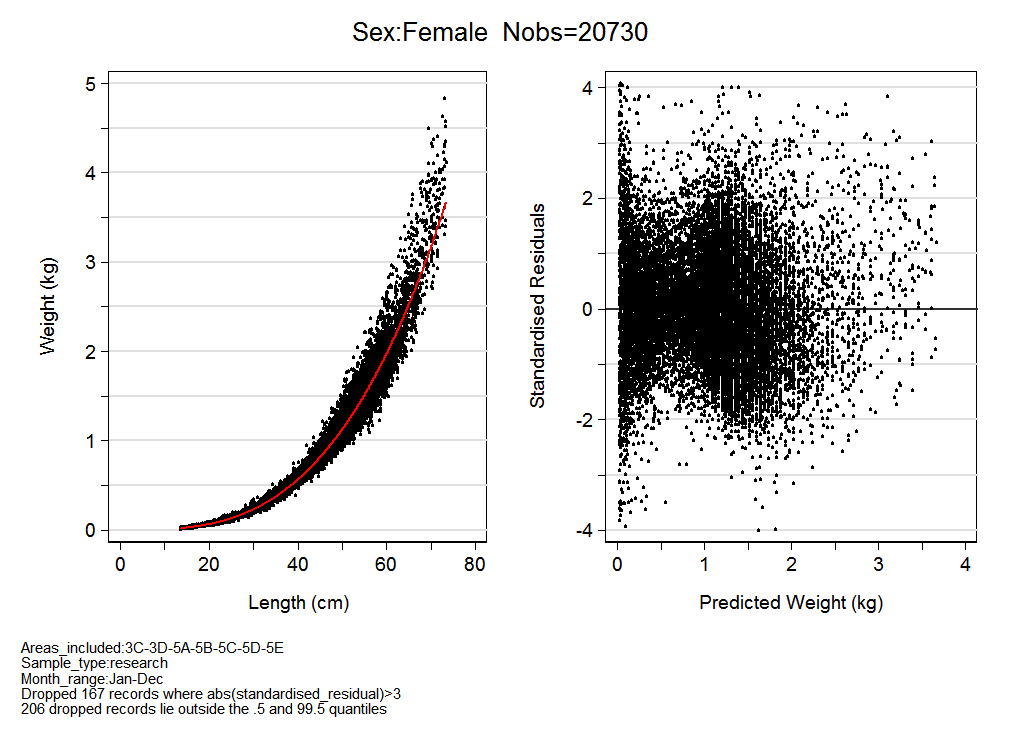
\includegraphics[bb=0 0 925 600,width=6in,keepaspectratio=true]{app-biology/lwfemaleOptionD.png}}
\end{center}
\caption{Length-weight plot for male [top panel] and female [bottom panel] \fishname: combined 3CD5ABCDE with standardised residuals \textgreater 3 discarded and with the lower 0.5 and upper 99.5 quantiles of length dropped (option D).}
\label{fig:lwOptionD}
\end{figure}

\begin{figure}[htp]
\captionsetup[subfigure]{labelformat=empty}
\begin{center}
\subfloat[]{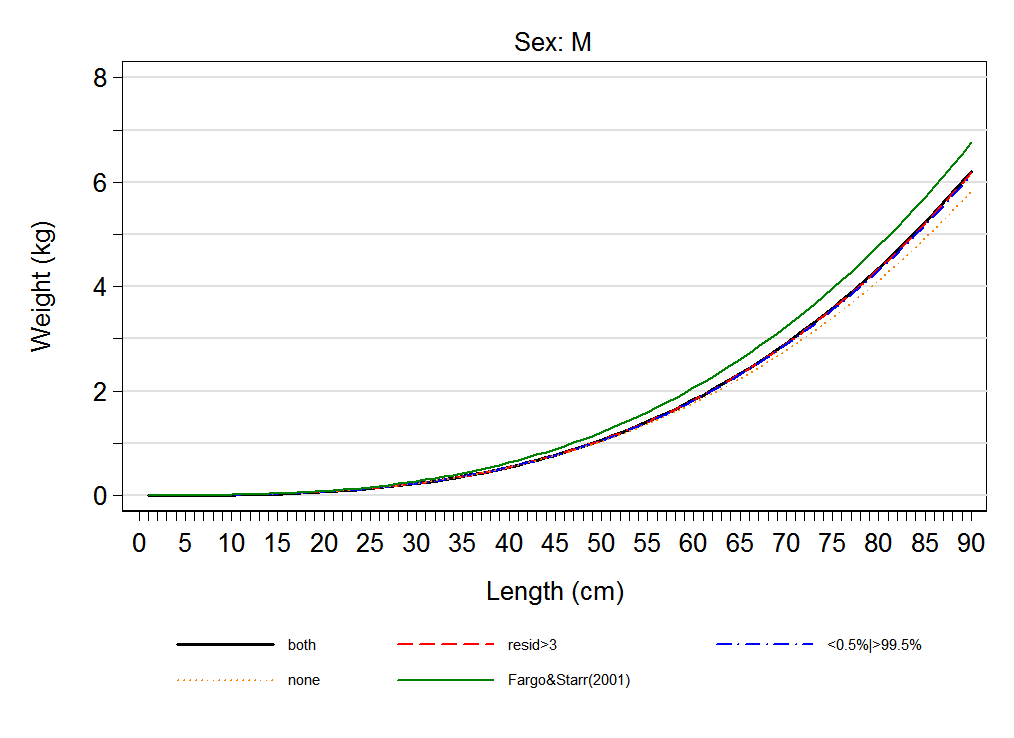
\includegraphics[bb=0 0 925 600,width=6in,keepaspectratio=true]{app-biology/lwmaleCompare.png}}
%\subfloat[]{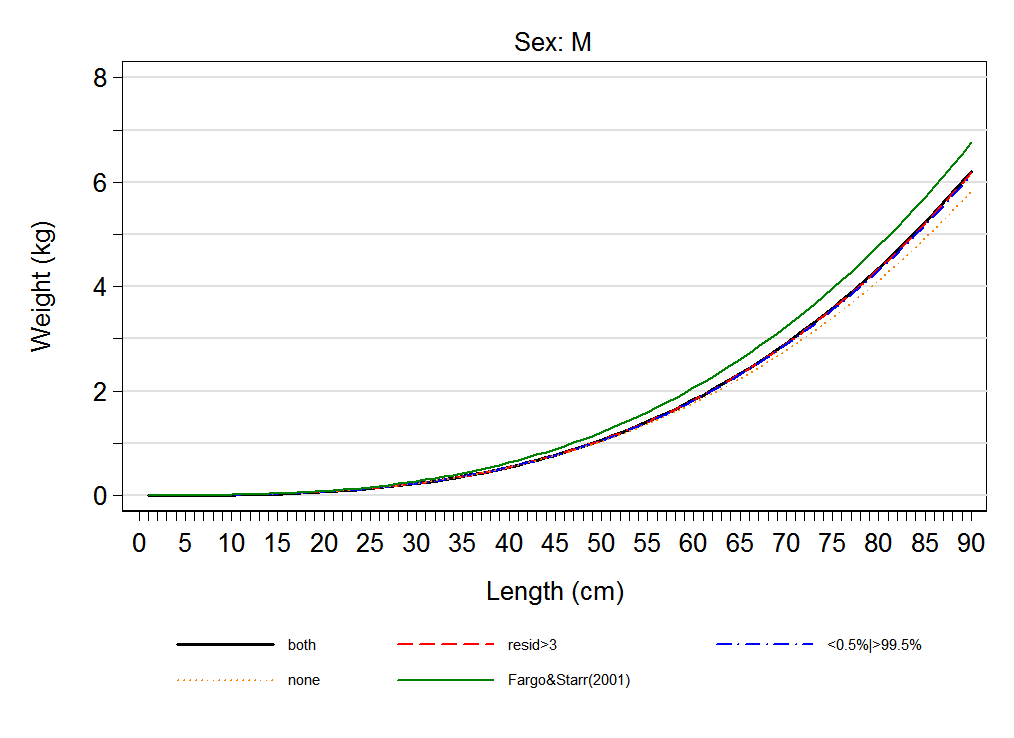
\includegraphics[angle=90, width=6in,keepaspectratio=true]{app-biology/lwmaleCompare.eps}}
\newline
\subfloat[]{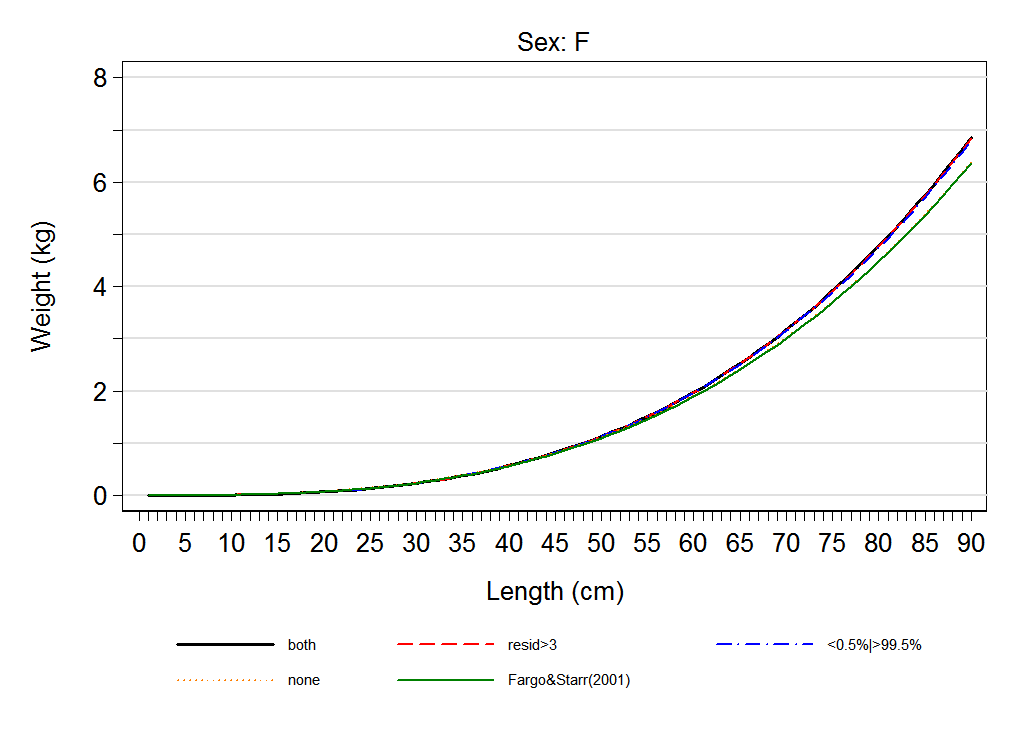
\includegraphics[bb=0 0 925 600,width=6in,keepaspectratio=true]{app-biology/lwfemaleCompare.png}}
%\subfloat[]{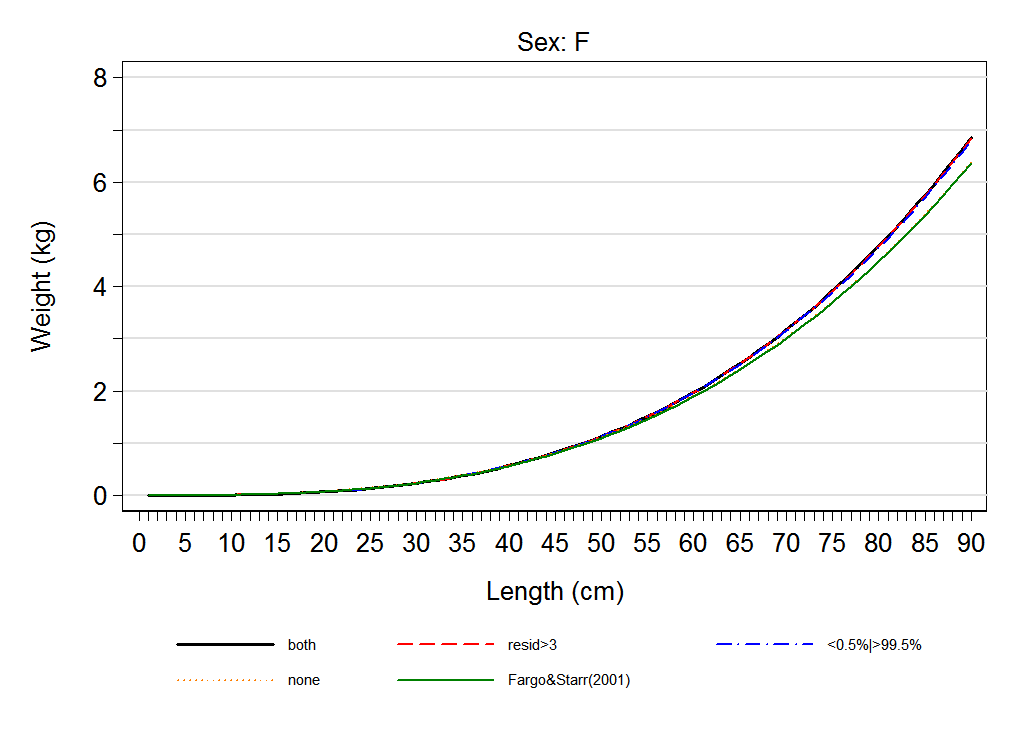
\includegraphics[angle=90, width=6in,keepaspectratio=true]{app-biology/lwfemaleCompare.eps}}
\end{center}
\caption{Comparative length-weight plots for male [top panel] and female [bottom panel] \fishname, showing the predicted power functions for the four models defined in Table~\ref{tab:bioCrit}. Also shown is the function by sex provided in Table 2 of \citet{arf2001}.}
\label{fig:lwCompare}
\end{figure}

\begin{figure}[htp]
\captionsetup[subfigure]{labelformat=empty}
\begin{center}
\subfloat[]{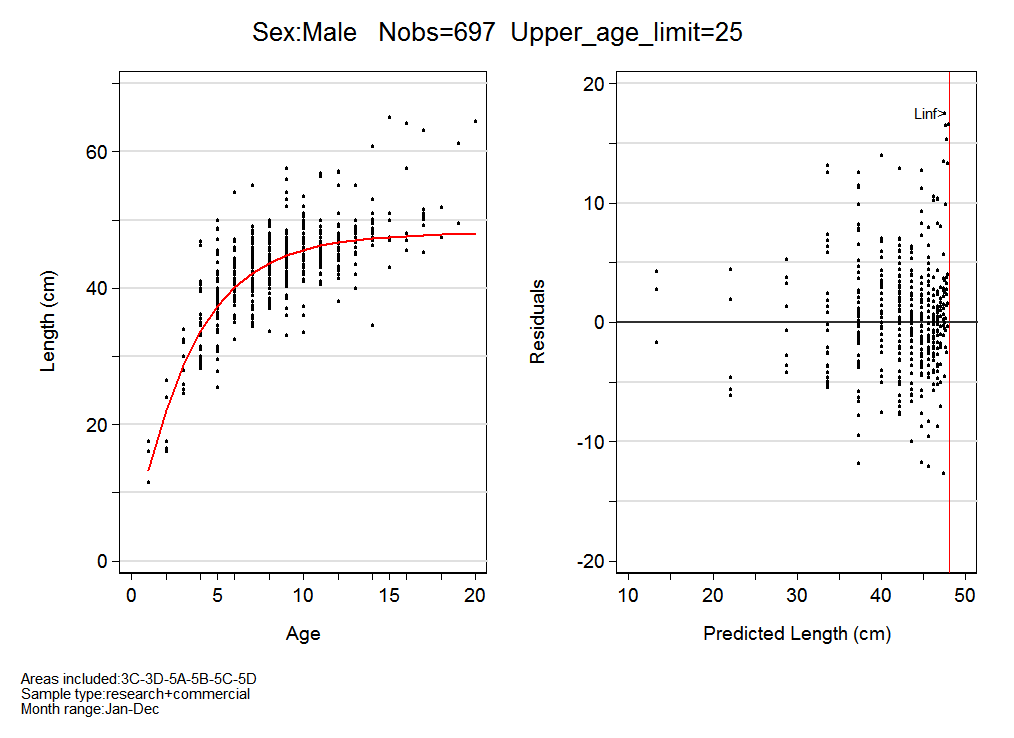
\includegraphics[bb=0 0 925 600,width=6in,keepaspectratio=true]{app-biology/vonbmale.png}}
\newline
\subfloat[]{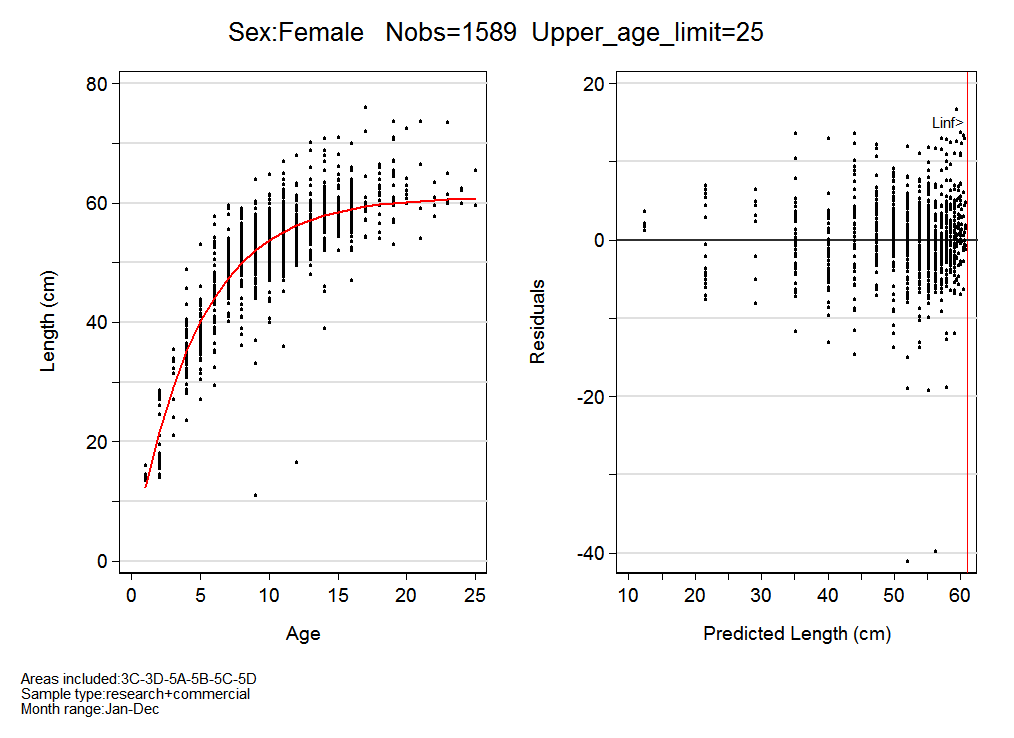
\includegraphics[bb=0 0 925 600,width=6in,keepaspectratio=true]{app-biology/vonbfemale.png}}
\end{center}
\caption{von-Bertalanffy plots for male [top panel] and female [bottom panel] \fishname: combined 3CD5ABCD using all available commercial and research data.}
\label{fig:vonb}
\end{figure}

\begin{figure}[htp]
\captionsetup[subfigure]{labelformat=empty}
\begin{center}
\subfloat[]{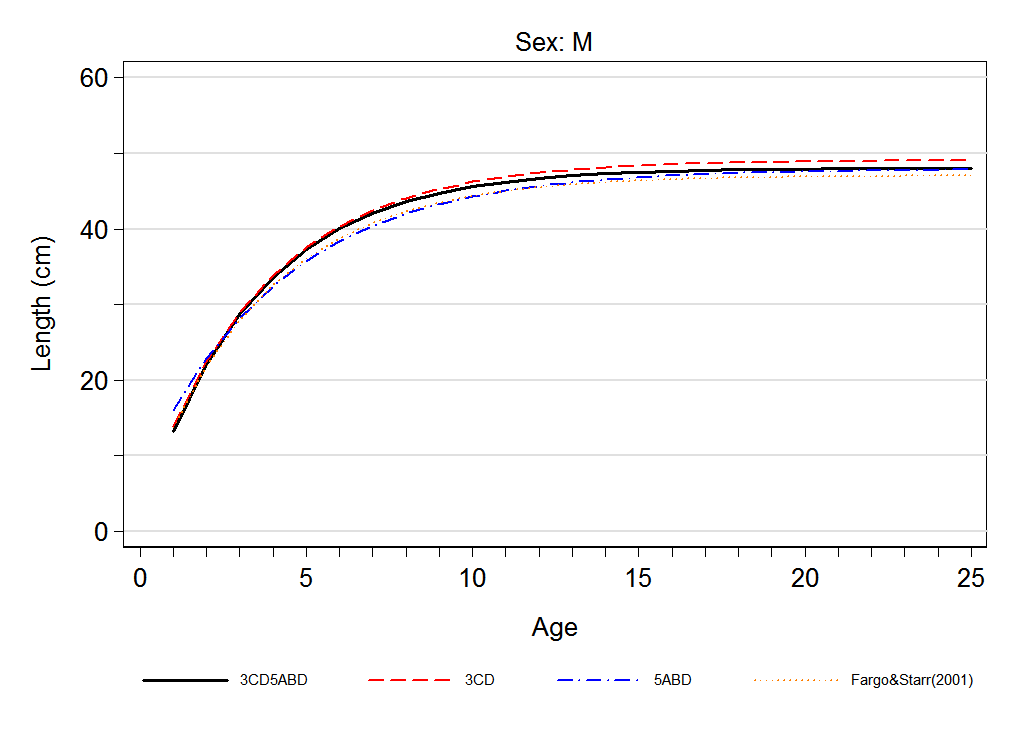
\includegraphics[bb=0 0 925 600,width=6in,keepaspectratio=true]{app-biology/vonbmaleCompare.png}}
\newline
\subfloat[]{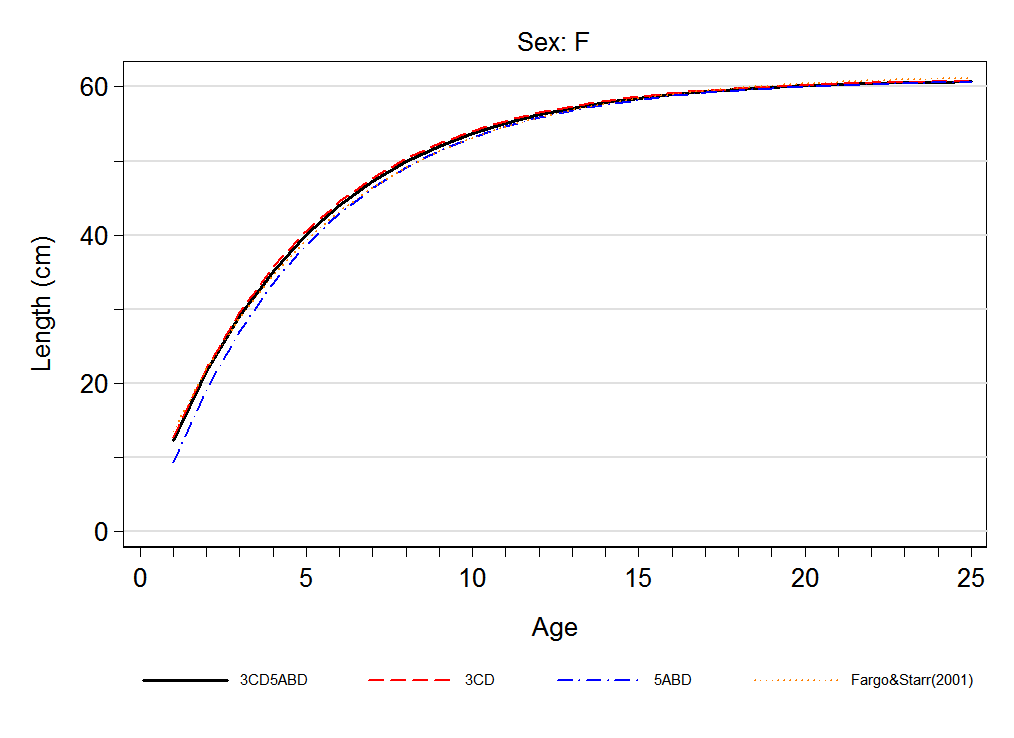
\includegraphics[bb=0 0 925 600,width=6in,keepaspectratio=true]{app-biology/vonbfemaleCompare.png}}
\end{center}
\caption{Comparative von-Bertalanffy plots for male [top panel] and female [bottom panel] \fishname, showing the predicted growth functions for the three models defined in Table~\ref{tab:vonbEst}.  Also shown is the function by sex provided in Table 2 of \citet{arf2001}.}
\label{fig:vonbCompare}
\end{figure}

\begin{figure}[htp]
\captionsetup[subfigure]{labelformat=empty}
\begin{center}
\subfloat[]{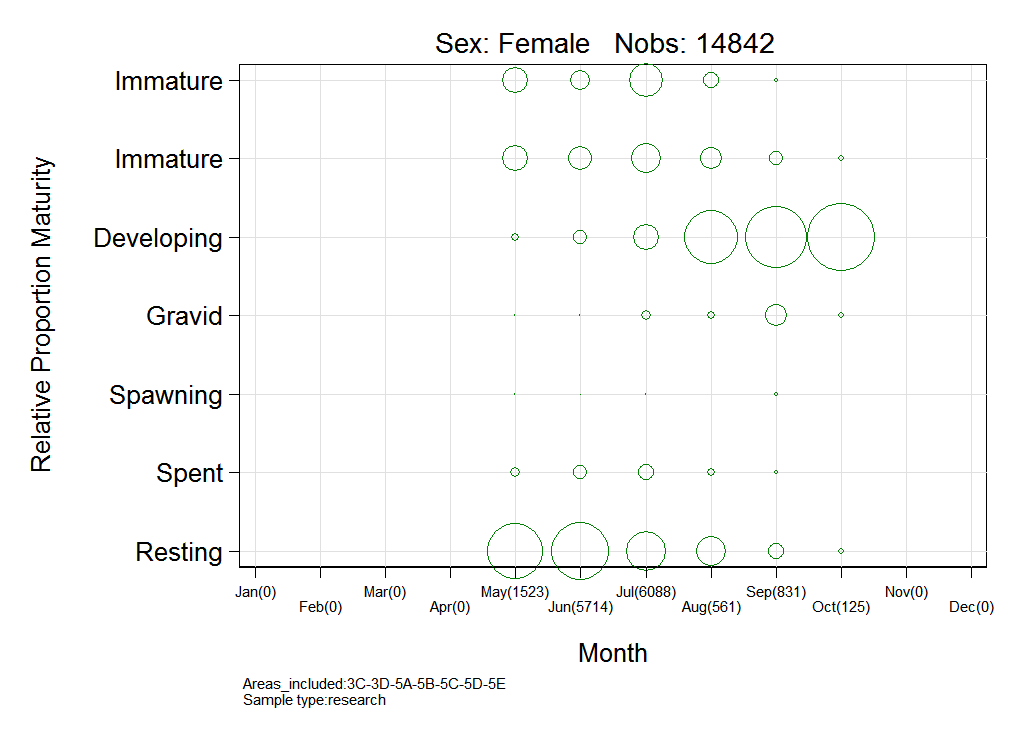
\includegraphics[bb=0 0 925 600,width=6in,keepaspectratio=true]{app-biology/maturityResearch.png}}
\newline
\subfloat[]{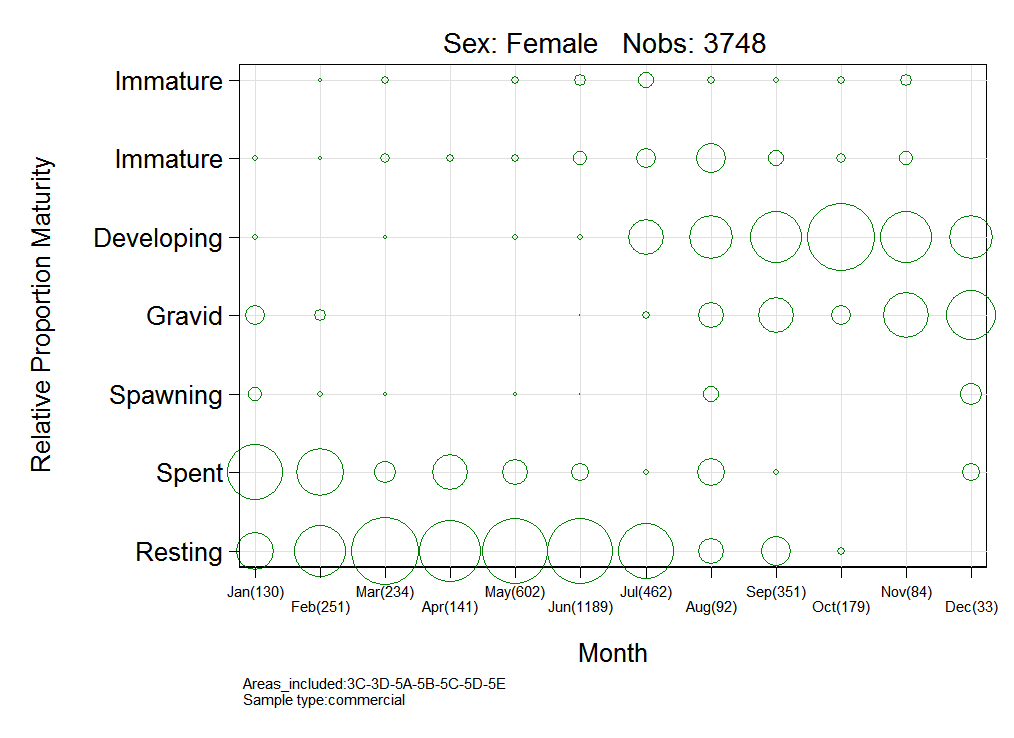
\includegraphics[bb=0 0 925 600,width=6in,keepaspectratio=true]{app-biology/maturityCommercial.png}}
\end{center}
\caption{Plots showing the proportion of \fishname females by maturity stage for each month; [top panel] research and charter survey observations [bottom panel] commercial observer observations. Each column sums to 1.0, with proportions provided in Table~\ref{tab:maturityMonth}}
\label{fig:maturity}
\end{figure}

\begin{figure}[htp]
\captionsetup[subfigure]{labelformat=empty}
\begin{center}
\subfloat[]{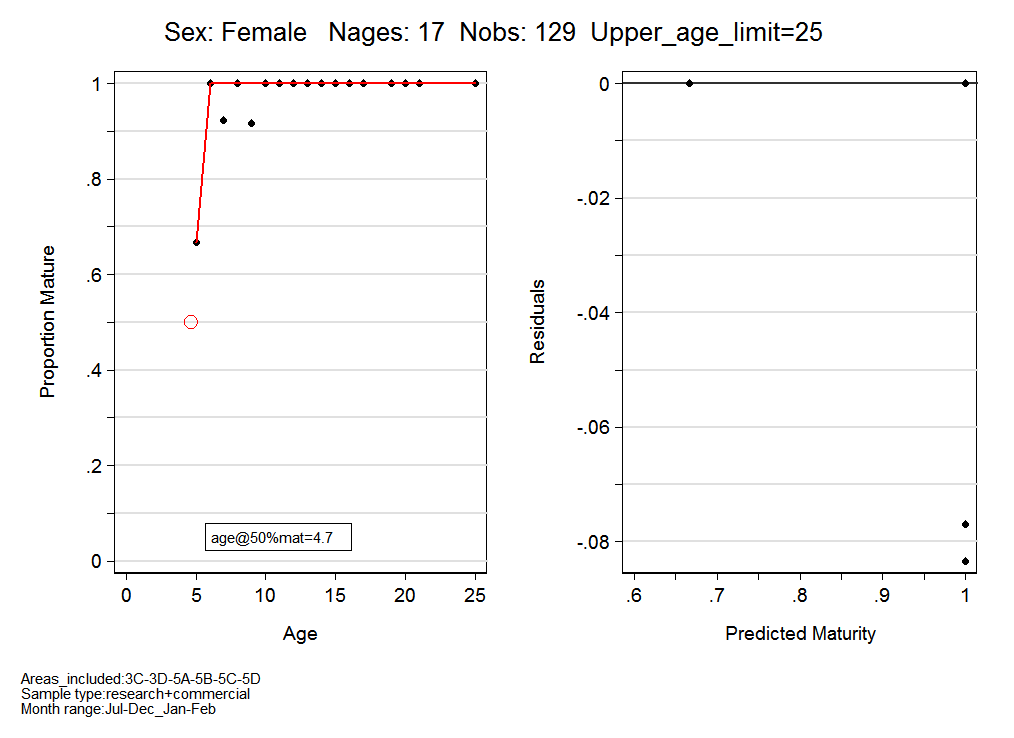
\includegraphics[bb=0 0 925 600,width=6in,keepaspectratio=true]{app-biology/maturityfitConstrainedMonths.png}}
\newline
\subfloat[]{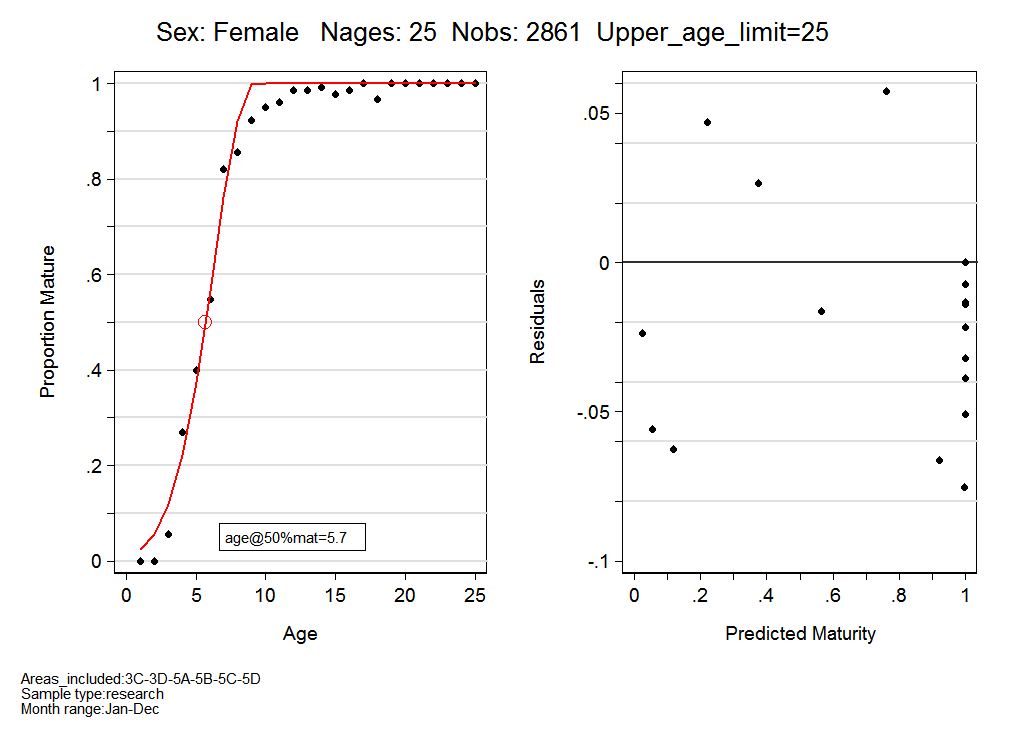
\includegraphics[bb=0 0 925 600,width=6in,keepaspectratio=true]{app-biology/maturityfitAllMonths.png}}
\end{center}
\vspace{-8mm}
\caption{Plots showing the observed proportions mature and the fitted maturity ogive by age for female \fishname: [top panel]: research and charter survey observations constrained to July-February; [bottom panel]: research observations from all months (January-November). The observed and fitted values by data source age, along with the number of otolith observations by age, are provided in Table~\ref{tab:maturityObsPred}.}
\label{fig:maturityfit}
\end{figure}

\begin{figure}[htp]
\captionsetup[subfigure]{labelformat=empty}
\begin{center}
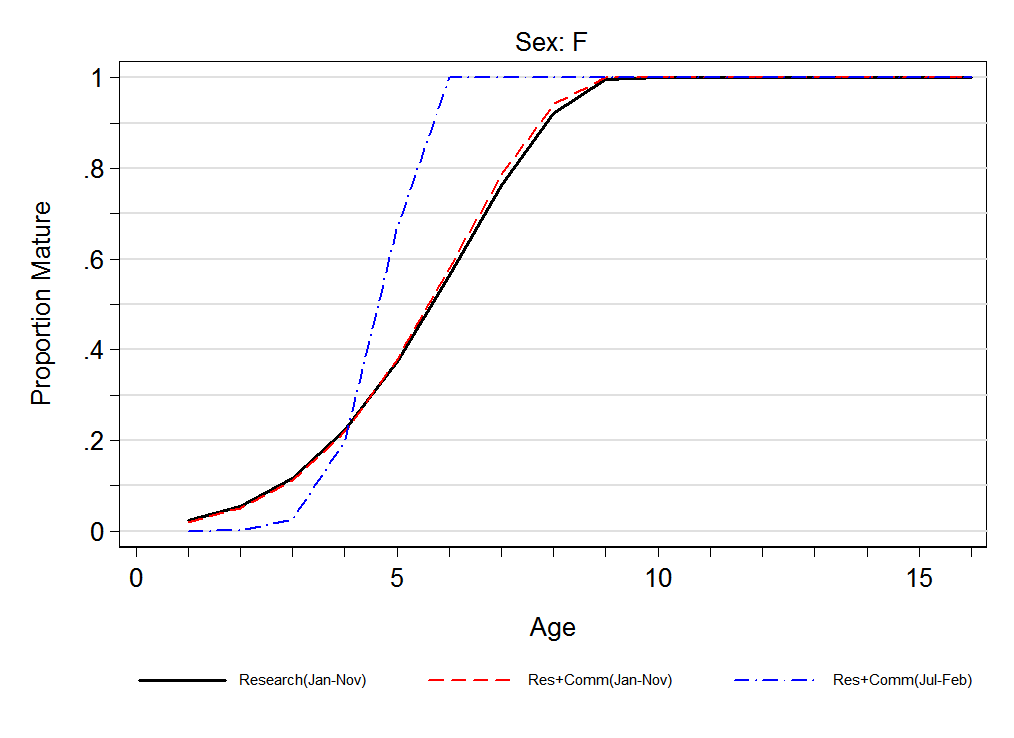
\includegraphics[bb=0 0 925 600,width=6in,keepaspectratio=true]{app-biology/maturityOgiveCompare.png}
\end{center}
\caption{Comparative maturity ogives for female \fishname, showing the predicted growth functions for the three models defined in Table~\ref{tab:parEst}.}
\label{fig:maturityOgiveCompare}
\end{figure}

\clearpage


% TABLES
\begin{table}[b]
\centering
\caption{\label{tab:bioCrit} Criteria for biological data extraction.}
\begin{tabular}{lrr}
\hline
Criterion & Notes \\
\hline
trip\_type==2 or trip\_type==3                               & definition of research observations \\
agemeth==3 or 17                                             & broken and burned or baked and broken \\
sample\_type==1 or 2 or 6 or 7                               & only random or total samples \\
month\textgreater=`startmonth' and month\textless=`endmonth' & valid month observation in range \\
sex==`sex'	                                                 & valid sex observation (1 or 2 ) \\
maturity\textgreater=1 and maturity\textless=7	             & valid maturity observation from 1 to 7 \\
select Not\_available\_reason\_code                          & not rejected \\
\hline
\end{tabular}
\end{table}

\begin{table}[b]
\tiny
\centering
\caption{\label{tab:lwEst} Length-weight parameter estimates, standard errors (SE) and number observations for male and female \fishname for all research observations in GFBio (trip\_type==2 or trip\_type==3) for combined PMFC Areas (3CD5ABCD) from 1989 to 2013. Restrictions are based on the distribution of residuals during a preliminary pass through data or on the empirical distribution of lengths by sex.}
\begin{tabular}{clcccccccc}
\hline
Option & Restrictions & \specialcell{N obs dropped\\residuals} & \specialcell{N obs dropped\\distribution} & \specialcell{N obs\\final} & $a^s$ & $b^s$ & SE($a^s$) & SE($b^s$) & $\bar{W}^s$ (kg) \\
\hline
Males \\
A & \specialcell{No distributional or residual\\restrictions} & 0 & 0 & 13,227 & -11.497 & 2.948 & 0.01600 & 0.00453 & 0.465 \\
B & \specialcell{No distributional restrictions\\residuals\textgreater3 dropped} & 79 & 0 & 13,148 & -11.714 & 3.009 & 0.00860 & 0.00243 & 0.465 \\
C & \specialcell{Lower 0.5\% and upper 99.5\%\\dropped, no residuals dropped} & 0 & 103 & 13,124 & -11.683 & 3.000 & 0.01121 & 0.00317 & 0.460 \\
D & \specialcell{Lower 0.5\% and upper 99.5\%\\dropped, residuals\textgreater3 dropped} & 127 & 103 & 12,997 & -11.732 & 3.014 & 0.00839 & 0.00237 & 0.461 \\
-- & \citet{arf2001} & -- & -- & -- & -11.270 & 2.930 & -- & -- & -- \\
\hline
Females \\
A & \specialcell{No distributional or residual\\restrictions} & 0 & 0 & 21,614 & -11.517 & 2.972 & 0.01560 & 0.00417 & 1.005 \\
B & \specialcell{No distributional restrictions\\residuals\textgreater3 dropped} & 55 & 0 & 21,559 & -11.871 & 3.066 & 0.00699 & 0.00186 & 1.005 \\
C & \specialcell{Lower 0.5\% and upper 99.5\%\\dropped, no residuals dropped} & 0 & 209 & 21,405 & -11.845 & 3.059 & 0.00883 & 0.00236 & 0.990 \\
D & \specialcell{Lower 0.5\% and upper 99.5\%\\dropped, residuals\textgreater3 dropped} & 168 & 209 & 21,237 & -11.890 & 3.071 & 0.00665 & 0.00177 & 0.992 \\
-- & \citet{arf2001} & -- & -- & -- & -11.600 & 2.993 & -- & -- & -- \\
\hline
\end{tabular}
\end{table}

\begin{table}[b]
\centering
\caption{\label{tab:numagesByArea} Number of paired length/observations by PMFC Region and sex. Also shows the maximum observed age by PMFC Region and sex.  Otoliths selected using criteria described in table~\ref{tab:bioCrit}.}
\begin{tabular}{lrrrr}
\hline
            & \multicolumn{2}{c}{Number ages} & \multicolumn{2}{c}{Maximum age} \\
\hline
PMFC region &  Male & Female &   Male & Female \\
\hline
3C          &   502 &    949 &     19 &     25 \\
3D          &   345 &    576 &     23 &     25 \\
5A          &     1 &      5 &     11 &     11 \\
5B          &    86 &    266 & 50$^1$ &     23 \\
5C          &   422 &    463 &     17 &     26 \\
5D          &   826 &  2,175 &     23 &     26 \\
5E          &    -- &     -- &     -- &     -- \\
Total       & 2,182 &  4,434 &     50 &     26 \\
$^1$ one observation only \\
\hline
\end{tabular}
\end{table}

\begin{table}[b]
\tiny
\centering
\caption{\label{tab:numagesByAreaMonth} Number of paired length/otolith observations by month and combined PMFC major region, showing the number of otoliths by sample source (Res=research or charter; Comm=observers aboard commercial vessels). Otoliths selected using criteria described in table~\ref{tab:bioCrit}.}
\begin{tabular}{|l|rrr|rrr|rrr|rrr|}
\hline
      & \multicolumn{3}{r|}{3CD} & \multicolumn{3}{r|}{5AB} & \multicolumn{3}{r|}{5CD} & \multicolumn{3}{r|}{Total Outside BC} \\
\hline
Month & Comm & Res & Total & Comm & Res & Total & Comm & Res & Total & Comm & Res & Total \\
\hline
January & 93 & -- & 93 & -- & -- & -- & -- & -- & -- & 93 & -- & 93 \\
February & 82 & -- & 82 & 1 & -- & 1 & -- & -- & -- & 83 & -- & 83 \\
March & 113 & -- & 113 & -- & -- & -- & 104 & -- & 104 & 217 & -- & 217 \\
April & 199 & -- & 199 & -- & -- & -- & -- & -- & -- & 199 & -- & 199 \\
May & 230 & 267 & 497 & 39 & -- & 39 & 404 & 354 & 758 & 673 & 621 & 1,294 \\
June & 223 & 1,051 & 1,274 & -- & 204 & 204 & 144 & 2,504 & 2,648 & 367 & 3,759 & 4,126 \\
July & 67 & -- & 67 & 30 & -- & 30 & 55 & -- & 55 & 152 & -- & 152 \\
August & -- & -- & -- & -- & -- & -- & -- & -- & -- & -- & -- & -- \\
September & -- & -- & -- & -- & -- & -- & 133 & -- & 133 & 133 & -- & 133 \\
October & 47 & -- & 47 & 49 & -- & 49 & 120 & -- & 120 & 216 & -- & 216 \\
Novermber & -- & -- & -- & 35 & -- & 35 & 68 & -- & 68 & 103 & -- & 103 \\
December & -- & -- & -- & -- & -- & -- & -- & -- & -- & -- & -- & -- \\
Total & 1,054 & 1,318 & 2,372 & 154 & 204 & 358 & 1,028 & 2,858 & 3,886 & 2,236 & 4,380 & 6,616 \\
\hline
\end{tabular}
\end{table}

\begin{table}[b]
\centering
\caption{\label{tab:vonbEst} von-Bertalanffy parameter estimates, standard errors (SE) and number observations for male and female \fishname for three models investigated for growth rate. Models in bold are the preferred models (plotted in Figure~\ref{fig:vonb}). These 3 models are superimposed by sex for comparison in Figure~\ref{fig:vonbCompare}.}
\begin{tabular}{lrrrrrrrr}
\hline
Option & Region & Nobs & $L_{\infty}^s$ & $k^s$ & $t_0^s$ & SE($L_{\infty}^s$) & SE($k^s$) & SE($t_0^s$) \\
\hline
Males \\
\textbf{Res+Comm} & \textbf{3CD5ABCD} & \textbf{2,181} & \textbf{50.13} & \textbf{0.239} & \textbf{-0.629} & \textbf{0.400} & \textbf{0.0105} & \textbf{0.1434} \\
Res+Comm & 3CD              & 847   & 51.96 & 0.237 & -0.453 & 0.712 & 0.0172 & 0.2524 \\
Res+Comm & 5ABCD            & 1,334 & 49.45 & 0.226 & -0.913 & 0.507 & 0.0126 & 0.1880 \\
 --      & \citet{arf2001}  & --    & 47.10 & 0.278 & -0.234 &    -- & --     & -- \\
Females \\
\textbf{Res+Comm} & \textbf{3CD5ABCD} & \textbf{4,432} & \textbf{61.65} & \textbf{0.190} & \textbf{-0.533} & \textbf{0.287} & \textbf{0.0042} & \textbf{0.0781} \\
Res+Comm & 3CD              & 1,525 & 62.84 & 0.191 & -0.427 & 0.459 & 0.0067 & 0.1372 \\
Res+Comm & 5ABCD            & 2,907 & 60.91 & 0.190 & -0.589 & 0.358 & 0.0053 & 0.0958 \\
 --      & \citet{arf2001}  & --    & 61.70 & 0.192 & -0.278 & --    & --     & -- \\
\hline
\end{tabular}
\end{table}

\begin{table}[b]
\tiny
\centering
\caption{\label{tab:maturityMonth} Proportion by maturity stage for each month for female \fishname, summed across all years for combined 3CD5ABCDE for A) research and charter boat observations; and B) commercial fishery observer observations. Each column sums to 1.0 for a month and sample type.}
\begin{tabular}{lrrrrrrrrrrrrr}
\hline
Stage      &   Jan &   Feb &   Mar &   Apr &   May &   Jun &   Jul &   Aug &   Sep &   Oct &   Nov &   Dec &  Total \\
\hline
\textbf{A) Research Observations} \\
Immature   &    -- &    -- &    -- &    -- & 0.146 & 0.087 & 0.238 & 0.053 & 0.002 &    -- &    -- &    -- &     -- \\
Immature   &    -- &    -- &    -- &    -- & 0.154 & 0.128 & 0.195 & 0.107 & 0.036 & 0.008 &    -- &    -- &     -- \\
Developing &    -- &    -- &    -- &    -- & 0.011 & 0.042 & 0.145 & 0.615 & 0.807 & 0.976 &    -- &    -- &     -- \\
Gravid     &    -- &    -- &    -- &    -- & 0.001 & 0.000 & 0.021 & 0.016 & 0.095 & 0.008 &    -- &    -- &     -- \\
Spawning   &    -- &    -- &    -- &    -- & 0.001 & 0.000 & 0.000 &    -- & 0.005 &    -- &    -- &    -- &     -- \\
Spent      &    -- &    -- &    -- &    -- & 0.018 & 0.040 & 0.057 & 0.012 & 0.004 &    -- &    -- &    -- &     -- \\
Resting    &    -- &    -- &    -- &    -- & 0.669 & 0.702 & 0.343 & 0.196 & 0.051 & 0.008 &    -- &    -- &     -- \\
N obs      &    -- &    -- &    -- &    -- & 1,577 & 6,171 & 6,088 &   561 &   831 &   125 &    -- &    -- & 15,353 \\
\hline
\textbf{B) Commercial Fishery Observations} \\
Immature   &    -- & 0.004 & 0.013 &    -- & 0.010 & 0.030 & 0.045 & 0.011 & 0.006 & 0.011 & 0.024 &    -- &     -- \\
Immature   & 0.008 & 0.004 & 0.017 & 0.014 & 0.013 & 0.042 & 0.076 & 0.163 & 0.051 & 0.022 & 0.036 &    -- &     -- \\
Developing & 0.008 &    -- & 0.004 &    -- & 0.008 & 0.007 & 0.253 & 0.380 & 0.527 & 0.877 & 0.536 & 0.364 &     -- \\
Gravid     & 0.069 & 0.032 &    -- &    -- &    -- & 0.001 & 0.011 & 0.120 & 0.248 & 0.078 & 0.405 & 0.485 &     -- \\
Spawning   & 0.038 & 0.008 & 0.004 &    -- & 0.003 & 0.001 &    -- & 0.054 &    -- &    -- &    -- & 0.091 &     -- \\
Spent      & 0.592 & 0.438 & 0.098 & 0.248 & 0.135 & 0.068 & 0.006 & 0.152 & 0.006 &    -- &    -- & 0.061 &     -- \\
Resting    & 0.285 & 0.514 & 0.863 & 0.738 & 0.831 & 0.851 & 0.608 & 0.120 & 0.162 & 0.011 &    -- &    -- &     -- \\
N obs      &   130 &   251 &   234 &   141 &   602 & 1,189 &   462 &    92 &   351 &   179 &    84 &    33 &  3,748 \\
\hline
\end{tabular}
\end{table}

\begin{table}[b]
\centering
\caption{\label{tab:maturityObsPred} Number of otoliths, observed and predicted maturities for the models (described in Table~\ref{tab:parEst}.) fitted to July--February and January--March.}
\begin{tabular}{|c|rrr|rrr|}
\hline
      & \multicolumn{3}{r|}{Res+Comm (Jul-Feb)} & \multicolumn{3}{r|}{Research (Jan-Nov)} \\
\hline
Age        & N\_otoliths & Obs\_mat & Pred\_mat & N\_otoliths & Obs\_mat & Pred\_mat \\
\hline
1  & -- &    -- &    -- &   6 &     0 & 0.024 \\
2  & -- &    -- &    -- & 121 &     0 & 0.056 \\
3  & -- &    -- &    -- &  91 & 0.055 & 0.117 \\
4  & -- &    -- &    -- & 108 & 0.269 & 0.221 \\
5  &  3 & 0.667 & 0.667 & 105 & 0.400 & 0.374 \\
6  &  2 &     1 &     1 & 126 & 0.548 & 0.564 \\
7  & 13 & 0.923 &     1 & 194 & 0.820 & 0.762 \\
8  & 12 &     1 &     1 & 318 & 0.855 & 0.922 \\
9  & 12 & 0.917 &     1 & 347 & 0.922 & 0.998 \\
10 & 20 &     1 &     1 & 374 & 0.949 &     1 \\
11 & 20 &     1 &     1 & 283 & 0.961 &     1 \\
12 & 12 &     1 &     1 & 213 & 0.986 &     1 \\
13 & 10 &     1 &     1 & 146 & 0.986 &     1 \\
14 & 13 &     1 &     1 & 137 & 0.993 &     1 \\
15 &  1 &     1 &     1 &  92 & 0.978 &     1 \\
16 &  3 &     1 &     1 &  74 & 0.986 &     1 \\
17 &  2 &     1 &     1 &  31 &     1 &     1 \\
18 &  2 &     1 &     1 &  31 & 0.968 &     1 \\
19 &  1 &     1 &     1 &  21 &     1 &     1 \\
20 &  2 &     1 &     1 &  19 &     1 &     1 \\
\hline
\end{tabular}
\end{table}

\begin{table}[b]
\centering
\caption{\label{tab:parEst} Parameter estimates with standard errors for three “double normal” models fitted to proportion mature by age fitting only the left-hand side variance and the age of full maturity (right-hand variance fixed such that maturity stays = 1.0. Also shown are the total number of otolith observations in each model and the derived parameter of median age of maturity ($^{50\%}a^f$).}
\begin{tabular}{llrrrrrr}
\hline
Data source & Month range & N\_otoliths & $A^f$ & ${\upsilon}L^f$ & SE($A^f$) & SE(${\upsilon}L^f$) & $^{50\%}a^f$ \\
\hline
Res+Comm    &     Jul-Feb &         129 &  6.00 &         0.903 &   0.0524 &            0.0000 &       4.69 \\
Res+Comm    &     Jan-Dec &       3,339 &  8.99 &         2.798 &   0.2259 &            0.1290 &       5.62 \\
Res         &     Jan-Nov &       2,861 &  9.21 &         2.891 &   0.2454 &            0.1336 &       5.68 \\
\hline
\end{tabular}
\end{table}

\clearpage


\rfoot{Appendix B -- Age Composition weighting}
\clearpage

\chapter{WEIGHTING OF AGE PROPORTIONS}
\label{chap:agecompweight}

This appendix summarizes a method for representing commercial and survey age structures for a given species through weighting observed age frequencies~$x_a$ or proportions~$x^\prime_a$ by \eor{catch}{density} in defined strata. 
(Throughout this section, we use the symbol \sQuote{$\Vert$} to delimit parallel values for commercial and survey analyses, respectively, as the mechanics of the weighting procedure are similar for both.) 
For commercial samples, these strata comprise quarterly periods within a year, while for survey samples, the strata are defined by longitude, latitude, and depth. 
Within each stratum, commercial ages are weighted by the catch weight (kg) of the species in tows that were sampled, and survey ages are weighted by the catch density (kg/km$^2$) of the species in sampled tows. 
A second weighting is then applied: quarterly commercial ages are weighted by the commercial catch weight of the species from all tows within each quarter; stratum survey ages are weighted by stratum areas (km$^2$) in the survey. 

Ideally, sampling effort would be proportional to the amount of the species caught, but this is not usually the case. 
Personnel can control the sampling effort on surveys more than that aboard commercial vessels, but the relative catch among strata over the course of a year or survey cannot be known with certainty until the events have occurred. 
Therefore, the stratified weighting scheme presented below attempts to adjust for unequal sampling effort among strata.

For simplicity herein, we illustrate the weighting of age frequencies~$x_a$, unless otherwise specified. 
The weighting occurs at two levels: $h$ (quarters for commercial ages, strata for survey ages) and $i$ (years if commercial, surveys in series if survey). 
Notation is summarised in Table~\ref{tab:wtdAges}.

\usefont{\encodingdefault}{\familydefault}{\seriesdefault}{\shapedefault}\small
\begin{longtable}[1]{l>{\raggedright\arraybackslash}p{0.85\textwidth} }
%\caption{Equations for weighting age frequencies or proportions for \fishname.\\(\bold{c})~= commercial, (\bold{s})~= survey}
\caption{Equations for weighting age frequencies or proportions for Arrowtooth Flounder.\\(\textbf{c})~= commercial, (\textbf{s})~= survey}
\label{tab:wtdAges} \\
\hline
Symbol & Description \\ %\tstrut \bstrut \\
\hline
%& \tstrut \textbf{Indices} \bstrut \\
& \textbf{Indices} \\
$\bM{a}$ & age class (1 to $A$, where $A$ is an accumulator age-class) \\
$\bM{d}$ & (\textbf{c}) trip IDs as sample units \\
& (\textbf{s}) sample IDs as sample units \\
$\bM{h}$ & (\textbf{c}) quarters (1 to 4), 91.5 days each \\
& (\textbf{s}) strata (area-depth combinations) \\
$\bM{i}$ & (\textbf{c}) calendar years (1977 to present) \\
& (\textbf{s}) survey IDs in survey series (e.g., QCS Synoptic) \\ %\bstrut \\
\hline
%& \tstrut \textbf{Data} \bstrut \\
& \textbf{Data} \\
$\bM{x_{adhi}}$ & observations-at-age $a$ for sample unit $d$ in \eor{quarter}{stratum} $h$ of \eor{year}{survey} $i$ \\
$\bM{x^\prime_{adhi}}$ & proportion-at-age $a$ for sample unit $d$ in \eor{quarter}{stratum} $h$ of \eor{year}{survey} $i$ \\
$\bM{C_{dhi}}$ & (\textbf{c}) commercial catch (kg) of a given species for sample unit $d$ in quarter $h$ of year $i$ \\
& (\textbf{s}) density (kg/km$^2$) of a given species for sample unit $d$ in stratum $h$ of survey $i$ \\
$\bM{C^\prime_{dhi}}$ & $C_{dhi}$ as a proportion of total \eor{catch}{density} $C_{hi} = \sum_{d} C_{dhi}$ \\
$\bM{y_{ahi}}$ & weighted age frequencies at age $a$ in \eor{quarter}{stratum} $h$ of \eor{year}{survey} $i$ \\
$\bM{K_{hi}}$ & (\textbf{c}) total commercial catch (kg) of species in quarter $h$ of year $i$ \\
& (\textbf{s}) stratum area (km$^2$) of stratum $h$ in survey $i$ \\
$\bM{K_{hi}^\prime}$ & $K_{hi}$ as a proportion of total \eor{catch}{area} $K_i = \sum_{h} K_{hi}$ \\
$\bM{p_{ai}}$ & weighted frequencies at age $a$ in \eor{year}{survey} $i$ \\
$\bM{p_{ai}^\prime}$ & weighted proportions at age $a$ in \eor{year}{survey} $i$ \\ %\bstrut \\
\hline 
% \end{tabular}
% \end{center}
\end{longtable}
\usefont{\encodingdefault}{\familydefault}{\seriesdefault}{\shapedefault}\normalsize

For each \eor{quarter}{stratum} $h$ we weight sample unit frequencies $x_{ad}$ by sample unit \eor{catch}{density} of the assessment species. (For commercial ages, we use trip as the sample unit, though at times one trip may contain multiple samples. In these instances, multiple samples from a single trip will be merged into a single sample unit.) Within any \eor{quarter}{stratum} $h$ and \eor{year}{survey} $i$ there is a set of sample \eor{catches}{densities} $C_{dhi}$ that can be transformed into a set of proportions:
%
\eqn{C_{dhi}^\prime = \gfrac{C_{dhi}}{\sum_{d} C_{dhi}}~.}
%
The proportion $C_{dhi}^\prime$ is used to weight the age frequencies $x_{adhi}$ summed over $d$, which yields weighted age frequencies by \eor{quarter}{stratum} for each \eor{year}{survey}:
%
\eqn{y_{ahi} = \sum_{d} \big(C_{dhi}^\prime x_{adhi}\big)~.}
%
This transformation reduces the frequencies $x$ from the originals, and so we rescale (multiply) $y_{ahi}$ by the factor
%
\eqn{\gfrac{\sum_{a} x_{ahi}}{\sum_{a} y_{ahi}}}
%
to retain the original number of observations. (For proportions $x^\prime$ this is not needed.) Although we perform this step, it is strictly not necessary because at the end of the two-step weighting, we standardise the weighted frequencies to represent proportions-at-age.

At the second level of stratification by \eor{year}{survey} $i$, we calculate the the annual proportion of quarterly catch (t) for commercial ages or the survey proportion of stratum areas (km$^2$) for survey ages
%
\eqn{K_{hi}^\prime = \gfrac{K_{hi}}{\sum_{h} K_{hi}}}
%
to weight $y_{ahi}$ and derive weighted age frequencies by \eor{year}{survey}:
%
\eqn{p_{ai} = \sum_{h} \big(K_{hi}^\prime y_{ahi}\big)~.}
%
Again, if this transformation is applied to frequencies (as opposed to proportions), it reduces them from the original, and so we rescale (multiply) $p_{ai}$ by the factor
%
\eqn{\gfrac{\sum_{a} y_{ai}}{\sum_{a} p_{ai}}~.}
%
to retain the original number of observations.

Finally, we standardise the weighted frequencies to represent proportions-at-age:
%
\eqn{p_{ai}^\prime = \gfrac{p_{ai}}{\sum_{a} p_{ai}}~.}
%
If initially we had used proportions $x_{adhi}^\prime$ instead of frequencies $x_{adhi}$ , the final standardisation would not be necessary; however, its application does not affect the outcome.

The choice of data input (frequencies $x$ \emph{vs}. proportions $x^\prime$) can sometimes matter: the numeric outcome can be very different, especially if the input samples comprise few observations. Theoretically, weighting frequencies emphasises our belief in individual observations at specific ages while weighting proportions emphasises our belief in sampled age distributions. Neither method yields inherently better results; however, if the original sampling methodology favoured sampling few fish from many tows rather than sampling many fish from few tows, then weighting frequencies probably makes more sense than weighting proportions. In this assessment, we weight age frequencies $x$.

\newpage


\rfoot{Appendix C -- Model Equations}
% appendix-equations.tex
% iSCAM model equations

\def\beq{\vspace{-5ex} \begin{fleqn} \begin{equation}}
\def\eeq{\end{equation} \end{fleqn} \vspace{-5ex}}
\def\tabline{\vspace{2ex} \hrule \vspace{2ex}}
\def\newp{\vfill \break}

\clearpage

\chapter{MODEL DESCRIPTION AND EQUATIONS}

\section{INTRODUCTION}

Stock Assessment modelling was conducted using the Integrated Statistical Catch Age Model (iSCAM), developed by Steven J.D. Martell (Martell et al. 2011).  iSCAM is written in AD Model Builder and the source code and documentation for the original iSCAM is available at https://github.com/smartell/iSCAM. Code for the version used in this assessment can be found at https://github.com/cgrandin/iSCAM. iSCAM uses a statistical catch-at-age model implemented in a Bayesian estimation framework.

Running of iSCAM and compilation of results figures was streamlined using the iscam-gui software package developed by Chris Grandin (pers. comm, Pacific Biological Station, Fisheries and Oceans Canada). iscam-gui is written in the statistical language R, and provides a graphical user interface that allows users to run and show output of multiple iSCAM model runs in a comparative fashion.

\section{MODEL DESCRIPTION}

This section contains the documentation in mathematical form of the underlying iSCAM age-structured model, and its steady state version that is used to calculate reference points, the observation models used in predicting observations, and the components of the objective function that formulate the statistical criterion (i.e. the objective function) that is used to estimate model parameters. All of the model equations are laid out in tables and are intended to represent the order of operations, or pseudocode, in which to implement the model. A documented list of symbols used in model equations is given in Table~\ref{tab:variables}. The documentation presented here is a revised version of the iscam user-guide written by S. Martell and available at https://github.com/smartell/iSCAM. Much of the text and equations have been taken directly from the original users guide.

\section{ANALYTIC METHODS: EQUILIBRIUM CONSIDERATIONS}

\subsection{A Steady-State Age-Structured Model}

For the steady-state conditions represented in Table~\ref{tab:model}, we assume the parameter vector $\Theta$ in Eq.~\ref{eq:df1} is unknown and would eventually be estimated by fitting iSCAM to data. For a given set of sex-specific growth parameters and maturity-at-age parameters defined by Eq.~\ref{eq:df2}, growth is assumed to follow von Bertalanffy (Eq.~\ref{eq:df3}), mean weight-at-age is given by the allometric relationship in Eq.~\ref{eq:df4}, and the age and sex-specific vulnerability is given by a age-based logistic function (Eq.~\ref{eq:df5}). There are alternative selectivity functions implemented in iSCAM; the age-based logistic function was used in this assessment.

Survivorship for unfished and fished populations is defined by Eqns.~\ref{eq:df7} and ~\ref{eq:df8}, respectively. Note that fished survivorship is sex-specific to allow for sex-specific $v_{a,s}$ when the age-based logistic function is used to model vulnerability. It is assumed that all individuals ages $A$ and older (i.e., the plus group) have the same total mortality rate. The incidence functions refer to the life-time or per-recruit quantities such as spawning biomass per recruit ($\phi_E$) or vulnerable biomass per recruit ($\phi_b$). Note that upper and lower case subscripts denote unfished and fished conditions, respectively. Spawning biomass per recruit is given by Eq.~\ref{eq:df9}, the vulnerable biomass per recruit is given by Eq.~\ref{eq:df10} and the per recruit yield to the fishery is given by Eq.~\ref{eq:df11}. Unfished recruitment is given by Eq.~\ref{eq:df12} and the steady-state equilibrium recruitment for a given fishing mortality rate $F_e$ is given by Eq.~\ref{eq:df13}. Note that in Eq.~\ref{eq:df13} we assume that recruitment follows a Ricker stock recruitment model of the form:

\[R_e=s_o R_e \phi_e e^{(-\beta R_e \phi_e)}\]
where the maximum juvenile survival rate is given by:
\[s_o=\frac{\kappa}{\phi_E},\]
and the density-dependent term is given by:
\[\beta=\frac{\ln\left(\kappa\right)}{R_{{o}}\phi_{{E}}},\]
which simplifies to Eq.~\ref{eq:df13}.

The equilibrium yield for a given fishing mortality rate is given by Eq.~\ref{eq:df14}. These steady-state conditions are critical for determining various reference points such as $F_{MSY}$ and $B_{MSY}$.

\subsection{MSY-based Reference Points}

When defining reference points for this assessment, only the current recreational fishery (with a 65cm size limit) was used to calculate MSY quantities. In the case of a single fishery such as this, iSCAM calculates $F_{MSY}$ by finding the value of $F_e$ that results in the zero derivative of \ref{eq:df14}. This is accomplished numerically using a Newton-Raphson method where an initial guess for $F_{MSY}$ is set equal to 1.0$M$. Given an estimate of $F_{MSY}$, other reference points such as MSY are calculated using the equations in Table~\ref{tab:model}.

A special class library to implement the MSY-based reference point calculations was developed specifically for iSCAM. Details of this algorithm, including partial derivatives for the numerical calculation of $F_{MSY}$, are available in the original iscam documentation available at: https://github.com/smartell/iSCAM.

%subsubsection{MSY-based Reference Points: Density-dependent $M$}

% %\newp % \baselineskip \mybaselineskip

\section{ANALYTIC METHODS: STATE DYNAMICS}

The estimated parameter vector in iSCAM is defined in Eq.~\ref{eq:df15} of Table~\ref{tab:model}. The unknown parameters $R_0$ and $\kappa$, as well as the fixed parameter $M$, are the leading population parameters that define the overall population scale. The total variance $\vartheta^2$ is estimated, while the proportion of the total variance that is associated with observation errors $\rho$ is assumed fixed. The total variance is partitioned into observation errors ($\sigma^2$) and process errors ($\tau^2$) using Eq.~\eqref{eq:df16}.

The unobserved state variables in Eq.~\eqref{eq:df17} include the numbers-at-age in year $t$ of sex $s$ ($N_{t,a,s}$), the spawning stock biomass in year $t$ of sex $s$ ($B_t$), and the total age- and sex-specific total mortality rate ($Z_{t,a,s}$).

The initial numbers-at-age in the first year (Eq.~\ref{eq:df18}) and the annual recruits (Eq.~\ref{eq:df19}) are treated as estimated parameters and used to initialize the numbers-at-age array. Recruitment at age-1 is assumed to be 50\% males and 50\% females. When a length-based selectivity function is used (i.e. for the Strait of Georgia Lingcod Recreational Fishery with a 65cm size limit; Table~\ref{tab:datasets}), age- and sex-specific selectivity for gear type $k$ is a function of the selectivity parameters ($a_k$ and $\gamma_k$, which represent length at 50\% selectivity and the associated standard deviation, respectively) and the sex-specific length-at-age $a$, $l_{a,s}$, as shown in Eq.~\ref{eq:df20}. For the two Strait of Georgia Lingcod fisheries modelled using age-based logisitc selectivity (Table~\ref{tab:datasets}), the $l_{a,s}$ variable in Eq.~\ref{eq:df20} is replaced with age $a$, and the selectivity parameters($a_k$ and $\gamma_k$) would be based on mean age of selectivity and the assocaited standard deviation. In this latter case, vulberability at age for these gears would be the same for males and females. The annual fishing mortality for each gear $k$ in year $t$ is the exponent of the estimated vector $\Gamma_{k,t}$ (Eq.~\ref{eq:df21}). The vector of log fishing mortality rate parameters $\Gamma_{k,t}$ is a bounded vector with a minimum value of -30 and an upper bound of 3.0. In arithmetic space this corresponds to a minimum value of 9.36e-14 and a maximum value of 20.01 for annual fishing mortality rates. In years where there are 0 reported catches for a given fleet, no corresponding fishing mortality rate parameter is estimated and the implicit assumption is there was no fishery in that year.

State variables in each year are updated using Eqns.~\ref{eq:df22}-~\ref{eq:df25}, where the spawning biomass is the product of the numbers-at-age and the mature biomass-at-age (Eq.~\ref{eq:df22}). The total mortality rate is given by Eq.~\ref{eq:df23}, and the total catch (in weight) for each gear is given by Eq.~\ref{eq:df24}, assuming that both natural and fishing mortality occur simultaneously throughout the year. Lingcod catch was not differentiated by sex, so both sexes were combined to calculate a total catch in Eq.~\ref{eq:df24}. The sex-specific numbers-at-age are propagated over time using Eq.~\ref{eq:df25}, where members of the plus group (age $A$) are all assumed to have the same total mortality rate.

Recruitment to age $k$ is assumed to follow a Beverton-Holt model for Arrowtooth Flounder (Eq.~\ref{eq:df26}) where the maximum juvenile survival rate ($s_o$) is defined by $s_o=\kappa/\phi_E$. For the Beverton-Holt model, $\beta$ is derived by solving Eq.~\ref{eq:df26} for $\beta$ conditional on estimates of $\kappa$ and $R_o$:
%\[
%\beta = \frac{\ln(\kappa)}{R_o \phi_E}
%\]

\section{RESIDUALS, LIKELIHOODS, AND OBJECTIVE FUNCTION VALUE COMPONENTS}

There are three major components to the overall objective function that are minimized while iSCAM is performing maximum likelihood estimation. These components consist of the likelihood of the data, prior distributions and penalty functions that are invoked to regularize the solution during intermediate phases of the non-linear parameter estimation. This section discusses each of these in turn, starting first with the residuals between observed and predicted states followed by the negative loglikelihood that is minimized.

\subsection{Catch data}

It is assumed that the measurement errors in the catch observations are log-normally distributed, and the residuals given by:
\begin{equation}\label{eq:df27}
\eta_{k,t}=\ln(C_{k,t}+o) -  \ln(\hat{C}_{k,t}+o),
\end{equation}
\begin{addmargin}[3em]{1em}
where $o$ is a small constant ($e^{-10}$) to ensure the residual is defined in the case of a 0 catch observation.
\end{addmargin}
The residuals are assumed to be normally distributed with a user-specified standard deviation $\sigma_{C}$.  At present, it is assumed that observed catches for each gear $k$  have the same standard deviation. The negative loglikelihood (ignoring the scaling constant) for the catch data is given by:
\begin{equation}\label{eq:df28}
\ell_C = \sum_k\left[  T_k\ln(\sigma_C)+\frac{\sum_t(\eta_{k,t})^2}{2\sigma_C^2}\right],
\end{equation}
where $T_k$ is the total number of catch observations for gear type $k$.

\subsection{Relative Abundance Data}

The relative abundance data are assumed to be proportional to biomass that is vulnerable to the sampling gear:
\begin{equation}\label{eq:df29}
 V_{k,t} = \sum_s \sum_a N_{t,a,s} e^{-\lambda_{k,t} Z_{t,a,s}} v_{k,a,s} w_{a,s},
\end{equation}
where $v_{k,a,s}$ is the sex- and age-specific selectivity of gear $k$, and $w_{a,s}$ is the mean-weight-at-age for sex $s$.  A user-specified fraction of the total mortality $\lambda_{k,t}$ adjusts the numbers-at-age to correct for survey timing. We set $\lambda_{k,t}$ to 0.5 for all index observations in the commercial and recreational CPUE indices since fishery catch and the collection of CPUE data are the same process, and natural mortality occures throughout the fishing season. 

\clearpage

\newp
% ********************** Table 1 ************************************
\begin{table}[b]
\centering
\caption{\label{tab:variables} A list of symbols, constants and description for variables used in iSCAM.}
\begin{tabular}{lll}
\hline
\bf{Symbol} & \bf{Value} & \bf{Description} \\
\hline
%\hline \ \\[-.5ex]
%
\multicolumn{3}{l}{\underline{Indices}}\\
$s$ & & Index for sex\\
$a$ & & Index for age\\
$t$ & & Index for year\\
$k$ & & Index for gear\\
\multicolumn{3}{l}{\underline{Model dimensions}}\\
$S$             & & Number of sexes\\
$\acute{a}, A$  & & Youngest and oldest age class ($A$ is a plus group)\\
$\acute{t}, T$  & & First and last year of catch data\\
$K$             & & Number of gears including survey gears\\
\multicolumn{3}{l}{\underline{Observations (data)}}\\
$C_{k,t}$        & & catch in weight by gear $k$ in year $t$\\
$I_{k,t}$        & & relative abundance index for gear $k$ in year $t$\\
%$p_{k,t,a}$     & & observed proportion-at-age $a$ in year $t$ for gear $k$\\
\multicolumn{3}{l}{\underline{Fixed parameters}}\\
$M_s$           & & Instantaneous natural mortality rate \\
%$M_{zero}$        & & Instantaneous natural mortality rate at zero abundance \\
$\rho$          & & Fraction of the total variance associated with observation error\\
$\vec{\gamma}_k$ & & Vector of selectivity parameters for gear $k$ \\
$\hat{a}_k, \hat{\gamma}_k$    &See Table~\ref{tab:datasets} & Selectivity parameters for gear $k$ \\
%$\lambda_{pow  \;  k}$ &See Table x.x & Exponent determining degree of denstiy-dependent catchability for gear $k$ \\
\multicolumn{3}{l}{\underline{Estimated parameters}}\\
$R_o$            & & Age-$\acute{a}$ recruits in unfished conditions\\
$\kappa$         & & Recruitment compensation\\
$\bar{R}$        & & Average age-$\acute{a}$ recruitment from year $\acute{t}$ to $T$\\
%$\ddot{R}$       & & Average age-$\acute{a}$ recruitment in year $\acute{t}-1$\\
$\vartheta$      & & Total precision (inverse of variance) of the total error\\
$\Gamma_{k,t}$    & & Logarithm of the instantaneous fishing mortality for gear $k$ in year $t$\\
%$\ddot{\omega}_a$   & & Age-$\acute{a}$ deviates from $\ddot{R}$ for year $\acute{t}$\\
$\omega_t$       & & Age-$\acute{a}$ deviates from $\bar{R}$ for years $\acute{t}$ to $T$\\
\multicolumn{3}{l}{\underline{Standard deviations}}\\
%$\sigma_M$       &0.1    & standard deviation in random walk for natural mortality\\
$\sigma$         & & Standard deviation for observation errors in survey index\\
$\tau$           & & Standard deviation in process errors (recruitment deviations)\\
$\sigma_C$       & & Standard deviation in observed catch by gear\\
\multicolumn{3}{l}{\underline{Residuals}}\\
$\delta_t$       &   & Annual recruitment residual\\
$\eta_t$         &   & Residual error in predicted catch\\
\multicolumn{3}{l}{\underline{Growth \& maturity parameters}}\\
$l_{\infty  s}$     & &  Asymptotic length in mm for males / females \\
$\acute{k}_s$    & & Brody growth coefficient for males / females \\
$t_{o s}$         & & Theoretical age at zero length for males / females \\
$\acute{a}_s$    & &  Scalar in length-weight allometry\\
$\acute{b}_s$    & & Power parameter in length-weight allometry for males / females\\
$\dot{a}_s$      & & Age at 50\% maturity for males / females \\
$\acute{\gamma}_s$ & & Standard deviation at 50\% maturity for males / females\\
\hline
\end{tabular}
\end{table}

\newp
% ********************** Table 2 ************************************
\begin{table}[b]
\centering
\caption{\label{tab:model} Steady-state age-structured model assuming unequal vulnerability-at-age, age-specific fecundity and Ricker type recruitment.}
\begin{tabular}{l}
\hline \\
\vbox{\begin{center}\bf{Parameters}\end{center}\vspace{-4ex}} \\
\vbox{\beq \Theta = (B_o,\kappa)\,; \ \ \ B_o>0; \kappa > 1 \label{eq:df1} \eeq} \\
\vbox{\beq \Phi = (l_{\infty,s},\acute{k}_s, t_{o,s},\acute{a}_s,\acute{b}_s,\dot{a}_s,\dot{\gamma}_s,\hat{a},\hat{\gamma}, M) \label{eq:df2} \eeq} \\
\\
\vbox{\begin{center}\bf{Age-schedule information}\end{center}\vspace{-4ex}} \\
\vbox{\beq l_{a,s}=l_{}\left(1-e^{\left(-k_s\left(a-t_{o,s}\right)\right)}\right) \label{eq:df3} \eeq} \\
\vbox{\beq w_{a,s}=\acute{a}_s(l_{a,s})^{\acute{b}_s} \label{eq:df4} \eeq} \\
\\
\vbox{\beq v_{a,s}=\left(1+e^{\left(\frac{-(\hat{a}-l_{a,s})}{\hat{\gamma}}\right)}\right)^{-1} \label{eq:df5} \eeq} \\
\\
\vbox{\beq f_{a,s}=w_{a,s}\left(1+e^{\left(\frac{-\left(\dot{a}_s-a\right)}{\dot{\gamma}_s}\right)}\right)^{-1} \label{eq:df6} \eeq} \\
\\
\vbox{\begin{center}\bf{Survivorship}\end{center}} \\
\vbox{\beq \iota_a = \begin{cases}
           \frac{1}{S}, & a = 1 \\
           \iota_{a-1}e^{-M}, & a > 1 \\
           \frac{\iota_{a-1}}{(1-e^{-M})}, & a = A \\
                     \end{cases}
      \label{eq:df7}
      \eeq} \\
\vspace{4ex} \\
\vbox{\beq \iota_a = \begin{cases}
           \frac{1}{S}, & a = 1 \\
           \hat{\iota}_{a-1,s}e^{-M-F_ev_{a-1,s}}, & a > 1 \\
           \frac{\hat{\iota}_{a-1,s}e^{-M-F_ev_{a-1,s}}}{(1-e^{-M-F_e v_{a,s}})}, & a = A \\
                     \end{cases}
      \label{eq:df8}
      \eeq} \\
\\
\vbox{\begin{center}\bf{Incidence functions}\end{center}} \\
\vbox{\beq \phi_E=\sum_{s=1}^S\sum_{a=1}^\infty \iota_a f_{a,s},\ \ \ \ \ \ \ \ \ 
           \phi_e=\sum_{s=1}^S\sum_{a=1}^\infty \hat{\iota}_{a,s} f_{a,s}
      \label{eq:df9}
      \eeq} \\
\vspace{2ex} \\
\vbox{\beq \phi_B=\sum_{s=1}^S\sum_{a=1}^\infty \iota_a w_{a,s} v_{a,s},\ \ \ 
           \phi_b=\sum_{s=1}^S\sum_{a=1}^\infty \hat{\iota}_{as} w_{a,s} v_{a,s}
      \label{eq:df10}
      \eeq} \\
\vspace{2ex} \\
\vbox{\beq \phi_q=\sum_{s=1}^S\sum_{a=1}^\infty
                  \frac{ \hat{\iota}_{a,s} w_{a,s} v_{a,s}}{M+F_ev_{a,s}}
                  \left(1-e^{(-M-F_ev_{a,s})}\right)
       \label{eq:df11}
       \eeq} \\
\vspace{1ex} \\
\vbox{\begin{center}\bf{Steady-state conditions}\end{center}\vspace{-4ex}} \\
\vbox{\beq R_o=\frac{B_o}{\phi_B} \label{eq:df12} \eeq} \\
\\
%% % For the next equation, if using Ricker, use:
%% \vbox{\beq R_e=R_o \dfrac{\ln(\kappa)-\ln(\phi_E/\phi_e)}{\ln(\kappa)}\ \ \ (Ricker) \label{eq:df13} \eeq} \\
%% % If using Beverton Holt, use:
%% \vbox{\beq R_e=R_o \dfrac{\kappa-\phi_E/\phi_e}{\kappa-1}  \label{df13} \eeq} \\
\vbox{\beq R_e=R_o \frac{\kappa-\frac{\phi_E}{\phi_e}}{\kappa-1}\ \ \ (Beverton-Holt) \label{eq:df13} \eeq} \\
\vbox{\beq C_e=F_e R_e \phi_q \label{eq:df14} \eeq} \\
\end{tabular}
\end{table}

\newp
%% % ********************** Table 3 ************************************

\begin{table}[b]
\centering
\caption{\label{tab:model} Statistical catch-age model using Baranov catch.}
\begin{tabular}{l}
\hline \\
\vbox{\begin{center}\bf{Estimated parameters}\end{center}\vspace{-4ex}} \\
\vbox{\beq \Theta= (R_0,\kappa,\bar{R},\vartheta^2,\Gamma_{k,t},\{\omega_t\}_{t=1-A}^{t=T})  \label{eq:df15} \eeq} \\
\\
\vbox{\beq \sigma^2=\frac{\rho}{\vartheta^2}, \;  \;  \; \; \tau^2=\frac{(1-\rho)}{\vartheta^2} \label{eq:df16} \eeq} \\
\vspace{2ex}
\\
\vbox{\begin{center}\bf{Unobserved states}\end{center}\vspace{-4ex}} \\
\\
\vbox{\beq N_{t,a},\; B_t,\; Z_{t,a}  \label{eq:df17} \eeq} \\
\vspace{2ex} \\
\vbox{\begin{center}\bf{Initial states}\end{center}\vspace{-4ex}} \\
\\
\vbox{\beq N_{t,a,s}=\frac{1}{S}\bar{R}e^{\omega_{t-a}} e^{-M^{\left(a-1\right)}};\ \ \ t=1;\ \ \ 2\leq a\leq A \label{eq:df18} \eeq} \\
\\
\vbox{\beq N_{t,a,s}=\frac{1}{S}\bar{R}e^{\omega_{t}};\ \ \ 1\leq t\leq T;\ \ \ a=1 \label{eq:df19} \eeq} \\
\\
\\
\vbox{\beq v_{k,a,s}= \frac{1}{1+e^{\left(-\frac{\left(l_{a,s} - \hat{a}_k\right)}{\hat{\gamma}_k}\right)}} \label{eq:df20} \eeq} \\
\\
\vbox{\beq  F_{k,t}=e^{\Gamma_{k,t}} \label{eq:df21} \eeq} \\
\\
\vbox{\begin{center}\bf{State dynamics ($t>1$)}\end{center}\vspace{-4ex}} \\
\\
\vbox{\beq  B_{t,s}=\sum_a N_{t,a,s}f_{a,s} \label{eq:df22} \eeq} \\
\\
\vbox{\beq  Z_{t,a,s}=M+\sum_k F_{k,t} v_{k,t,a,s}  \label{eq:df23} \eeq} \\
\\
\vbox{\beq \hat{C}_{k,t}=\sum _ s\sum _ a\frac {N_{{t,a,s}}w_{{a,s}}F_{k,t} v_{{k,t,a,s}} \left( 1-{e^{-Z_{t,a,s}}} \right) }{Z_{t,a,s}}^{\eta_t}  \label{eq:df24} \eeq} \\
\vspace{4ex} \\
\vbox{\beq N_{t,a,s} = \begin{cases}
           \frac{s_oE_{t-1}}{1+\beta E_{t-1}} e^{(\omega_t-0.5\tau^2)} & a=1 \\
           N_{t-1,a-1,s} e^{(-Z_{t-1,a-1,s})} &a>1 \\
           N_{t-1,a,s} e^{(-Z_{t-1,a,s})} & a=A \\
                      \end{cases}
       \label{eq:df25}
       \eeq} \\
\\
\vbox{\begin{center}\bf{Recruitment model}\end{center}\vspace{-4ex}} \\
\\
\\
%% % If using Ricker:
%% \vbox{\beq R_t = s_oB_{t-k}e^{-\beta B_{t-k}+\delta_t-0.5\tau^2}\ \ \  (Ricker) \label{df26} \eeq} \\
%% % If using Beverton-Holt:
%% \vbox{%\beq R_t = \frac{s_oB_{t-k}}{1+\beta B_{t-k}}e^{\delta_{t}-0.5\tau^2} \label{df26} \eeq} \\
\vbox{\beq R_t = \frac{s_oB_{t-k}}{1+\beta B_{t-k}}e^{\delta_{t}-0.5\tau^2}\ \ \ (Beverton-Holt) \label{eq:df26} \eeq} \\

\end{tabular}
\end{table}

\newp
%% % ********************** Table 4 ************************************
\begin{table}[b]
\centering
\caption{\label{tab:datasets} Definition of datasets denoted by gear index $k$ in Tables~\ref{tab:variables} - ~\ref{tab:model}}
\begin{tabular}{lllccc}
\hline \\
$k$  & Dataset & \specialcell{Years with\\catch data} & \specialcell{Selectivity\\type} & \specialcell{Selectivity\\parameters} \\   %($\hat{a}, \hat{\gamma}$ ) \\
\hline \\
1 & Commercial fishery     & 1996-2014             & Age-based & TODO \\
2 & WCVI Synoptic survey   & 2004-2014 (even)      & Age-based & TODO \\
3 & HS Synoptic survey     & 2005-2013 (odd)       & Age-based & TODO \\
4 & HS Assemblage survey   & 2005-2013 (odd)       & Age-based & TODO \\
5 & QCS Synoptic survey    & 2003-2013 (odd+2004)  & Age-based & TODO \\
6 & HS Synoptic survey     & 2005-2013 (odd)       & Age-based & TODO \\
7 & WCVI Shrimp survey     & 1996-2014             & Age-based & TODO \\
8 & QCS Shrimp survey      & 1999-2013             & Age-based & TODO \\
\hline \\
\end{tabular}
\end{table}


%% \section{RESIDUALS, LIKELIHOODS, AND OBJECTIVE FUNCTION VALUE COMPONENTS}

%% There are three major components to the overall objective function that are minimized while iSCAM is performing maximum likelihood estimation.  These components consist of the likelihood of the data, prior distributions and penalty functions that are invoked to regularize the solution during intermediate phases of the non-linear parameter estimation.  This section discusses each of these in turn, starting first with the residuals between observed and predicted states followed by the negative loglikelihood that is minimized.

%% \subsection{Catch Data}

%% It is assumed that the measurement errors in the catch observations are log-normally distributed, and the residuals given by:
%% \begin{equation}\label{df27}
%% \eta_{k,t}=\ln(C_{k,t}+o) -  \ln(\hat{C}_{k,t}+o),
%% \end{equation}
%% \begin{addmargin}[3em]{1em}
%% where $o$ is  a small constant (1.e-10) to ensure the residual is defined in the case of a 0 catch observation.
%% \end{addmargin}
%% The residuals are assumed to be normally distributed with a user-specified standard deviation $\sigma_{C}$.  At present, it is assumed that observed catches for each gear $k$  have the same standard deviation.  The negative loglikelihood (ignoring the scaling constant) for the catch data is given by:
%% \begin{equation}\label{df28}
%% \ell_C = \sum_k\left[  T_k\ln(\sigma_C)+\frac{\sum_t(\eta_{k,t})^2}{2\sigma_C^2}\right],
%% \end{equation}
%% \begin{addmargin}[3em]{1em}
%% where $T_k$ is the total number of catch observations for gear type $k$.
%% \end{addmargin}

%% Commercial fishery catch data for Area 4B Lingcod are available in biomass units (tonnes), while catch from recreational fisheries are reported as numbers (pieces).  iSCAM allows users to specify catch units as biomass or numbers; however, to accomodate the constraint that catches from all gears have the same standard deviation, we re-scale recreational catch to 10's of pieces so that it would be on the same scale as catch in tonnes from the commercial fishery.  This re-scaling required us to specifythe parameters for the allometric weight-length relationship in \ref{eq:df4} in units of mm to 100's of kg.

%% \subsection{Relative Abundance Data}

%% The relative abundance data are assumed to be proportional to biomass that is vulnerable to the sampling gear:
%% \begin{equation}\label{df29}
%%  V_{k,t} = \sum_s \sum_a N_{t,a,s} e^{-\lambda_{k,t} Z_{t,a,s}} v_{k,a,s} w_{a,s},
%% \end{equation}
%% \begin{addmargin}[3em]{1em}
%% where $v_{k,a,s}$ is the sex- and age-specific selectivity of gear $k$, and $w_{a,s}$ is the mean-weight-at-age for sex $s$.
%% \end{addmargin}
%% A user-specified fraction of the total mortality $\lambda_{k,t}$ adjusts the numbers-at-age to correct for survey timing.  We set $\lambda_{k,t}$ to 0.5 for all index observations in the commercial and recreational CPUE indices since fishery catch and the collection of CPUE data are the same process, and natural mortality occures throughout the fishing season. 

%% The residuals between the observed and predicted relative abundance index is given by:
%% \begin{equation}\label{df30}
%% \epsilon_{k,t} = \ln(I_{k,t}) - \ln(q_k)+\ln(V_{k,t}),
%% \end{equation}
%% \begin{addmargin}[3em]{1em}
%% where $I_{k,t}$ is the observed relative abundance index, $q_k$ is the catchability coefficient for index $k$, and $V_{k,t}$ is the predicted vulnerable biomass at the time of sampling.
%% \end{addmargin}
%% The catchability coefficient $q_k$ is evaluated at its conditional maximum likelihood estimate:
%% \[
%%   q_k =\frac{1}{N_k} \sum_{t \in I_{k,t}} \ln(I_{k,t}) - \ln(V_{k,t}),
%% \]
%% where $N_k$ is the number of relative abundance observations for index $k$ (see Walters and Ludwig 1994 for more information). The negative loglikelihood for relative abundance data is given by:
%% \begin{align}
%% \ell_I &= \sum_k \sum_{t \in I_{k,t}}  \ln(\sigma_{k,t})+\frac{\epsilon_{k,t}^2}{2\sigma_{k,t}^2} \label{df31}\\
%% &\mbox{where}\nonumber\\
%% \sigma_{k,t} &= \frac{\rho \varphi^2}{ \omega_{k,t}},  \nonumber
%% \end{align}
%% \begin{addmargin}[3em]{1em}
%% where $\rho \varphi^2$ is the proportion of the total error that is associated with observation errors, and $\omega_{k,t}$ is a user specified relative weight for observation $t$ from gear $k$. The $ \omega_{k,t}$ terms allow each observation to be weighted relative to the total error $\rho \varphi^2$; for example, to omit a particular observation, set $\omega_{k,t}=0$, or to give 2 times the weight, then set  $\omega_{k,t}=2.0$.
%% \end{addmargin}
%% For the current assessment, we assumed all observations have the same variance by setting  $\omega_{k,t}=1$.  Note that if  $\omega_{k,t}=0$ then equation \ref{eq:df31} is undefined; therefore, iSCAM adds a small constant to $\omega_{k,t}$ (1e-10), which is equivalent to assuming an extremely large variance) to ensure the likelihood can be evaluated.

%% \vspace{2ex}
%% \subsubsection{Option for Non-linear CPUE Relationship}

%% The option to model relative abundance indices as a power function of vulnerable biomass was added to the version of iSCAM used for this assessment to allow replication of the approach taken in the last Strait of Gerogia Lingcod assessment (Logan et al. 2005).  This approach was taken in 2005 because the qualified commercial CPUE index used as an abunance index was not expected to be linearly related to abundance.  In this case, \ref{eq:df29} is replaced by:      
%% \begin{equation}\label{df32}
%%  V_{k,t} = (\sum_s \sum_a N_{t,a,s} e^{-\lambda_{k,t} Z_{t,a,s}} v_{k,a,s} w_{a,s})^{\psi_k}
%% \end{equation}
%% where $\psi_k$ is an exponent determining the degree of linearity between the CPUE series from gear $k$ and the vulnerable biomass available to gear $k$ in year $t$.  When $\psi_k$ is less than 1, a given change in CPUE implies a greater relative change in exploitable abundance (hyperstability); when $\psi_k$ = 1, CPUE is proportional to abundance; and when $\psi_k$ is greater than 1, a given change in CPUE implies a lesser relative chance in abundance (hyperdepletion).  The $\psi_k$ parameters for each gear $k$ were estimated by Logan et al. (2005); however, we did not attempt to estimate these in our bridging analysis due to concerns of model overparameterization.  Instead, $\psi_k$ was fixed at the values estimated by Logan et al. (2005) in scenarios that used a non-linear CPUE relationship (Table~\ref{tab:fixedExponentValues}.


%% % ********************** Table 5 ************************************
%% \begin{table}[tp]
%% \leftskip=1.5em
%% \parindent=-1.5em
%% \caption{\label{tab:fixedExponentValues} Fixed values used for exponent determining degree of linearity between vulnerable biomass and commercial CPUE (cCPUE) or recreational CPUE (rCPUE) series ($\psi_k$  in \ref{eq:df32}) when non-linear CPUE option selected.  Values are given for three different scenarios about the treatment of historic catch values in SubAreas 28 and 29 (i.e., the southeast quadrant).}
%% %\vsd \\
%% \leftskip=0em
%% \parindent=-0em
%% \begin{center}
%% \begin{tabular}{lcc} 
%% \hline \\[-1.5ex]
%% Scenario   &   $\psi_{cCPUE}$       &    $\psi_{rCPUE}$   \\ 
%% \hline %\\[-.5ex]
%% SoG & 0.878 & 1.759 \\
%% noSE & 0.646 & 0.611 \\
%% halfSE & 0.878 & 1.759 \\
%% \hline 
%% \end{tabular} 
%% \vsd
%% \end{center}
%% \end{table}


%% %\subsub{Relative Age composition Data}
%% %
%% % krHolt Note: The following text will require a few tweaks to get it to work in this template.  Is taken directly from Steve's iscam documentation.
%% %
%% %Sampling theory suggest that age composition data are derived from a multinomial distribution \citep{fournier1982general}; however, \iscam\ assumes that age-proportions are obtained from a multivariate logistic distribution \citep{schnute1995influence,richards1997visualizing}.  The main reason \iscam\ departs from the traditional multinomial model has to do with how the age-composition data are weighted in the objective function.  First, the multinomial distribution requires the specification of an effective sample size; this may be done arbitrarily or through iterative re-weighting \citep{MCALLISTER1997,gavaris2002sif}, and in the case of multiple and potentially conflicting age-proportions this procedure may fail to converge properly.  The assumed effective sample size can have a large impact on the overall model results.  
%% %
%% %A nice feature of the multivariate logistic distribution is that the age-proportion data can be weighted based on the conditional maximum likelihood estimate of the variance in the age-proportions.  Therefore, the contribution of the age-composition data to the overall objective function is ``self-weighting'' and is conditional on other components in the model.
%% %
%% %Ignoring the subscript for gear type for clarity, the observed and predicted proportions-at-age must satisfy the constraint 
%% %\[
%% % \sum_{a=1}^A p_{t,a} = 1
%% %\]
%% %for each year. The residuals between the observed ($p_{t,a}$) and predicted proportions ($\widehat{p_{t,a}}$) is given by:
%% %\begin{equation}\label{eq7}
%% %\eta_{t,a}=\ln(p_{t,a})-\ln(\widehat{p_{t,a}})-\frac{1}{A}\sum_{a=1}^A\left[\ln(p_{t,a})-\ln(\widehat{p_{t,a}}) \right].
%% %\end{equation}
%% %The conditional maximum likelihood estimate of the variance is given by
%% %\[
%% %\widehat{\tau}^2=\frac{1}{(A-1)T}\sum_{t=1}^T\sum_{a=1}^A \eta_{t,a}^2,
%% %\]
%% %and the negative loglikelihood evaluated at the conditional maximum likelihood estimate of the variance is given by:
%% %\begin{equation}\label{eq8}
%% %    \ell_A = (A-1)T \ln(\widehat{\tau}^2).
%% %\end{equation}
%% %In short, the multivariate logistic likelihood for age-composition data is just the log of the residual variance weighted by the number observations over years and ages.
%% %
%% %%Add technical details about requiring the minimum p_{t,a} to be greater than 2% "Grouping".
%% %There is also a technical detail in \ref{eq:eq7}, where observed and predicted proportions-at-age must be greater than 0.  It is not uncommon in catch-age data sets to observe 0 proportions for older, or young, age classes.  \iscam\ adopts the same approach described by \cite{richards1997visualizing} where the definition of age-classes is altered to require that $p_{t,a}\geq 0.02$ for every age in each year.  This is accomplished by grouping consecutive ages, where $p_{t,a} <0.02$, into a single age-class and reducing the effective number of age-classes in the variance calculation ($\widehat{\tau}^2$) by the number of groups created.  The choice of 2\% is arbitrary and the user can specify the minimum proportion (including 0) to consider when pooling age-proportion data.  In the case of an exact 0 in the observed age-proportions the pooling of the adjacent age-class still occurs, this ensures that \ref{eq:eq7} is defined.
%% %
%% %
%% %A \textbf{WARNING} about extremely weak year classes is required here.  A potential problem exists if in fact there is a very small cohort relative to the adjacent cohorts such that it never makes up more than say 2\% (or whatever minimum is specified) of the age-proportions in any given year.  In such cases, the information in the age-composition data about this weak year class relative to of that the adjacent (younger) year class because its always pooled into the younger year class.  \iscam\ will actually estimate two strong cohorts instead of correctly estimating one strong and one weak cohort in the following year.


%% \subsection{Stock-Recruitment}

%% Annual recruitment and the initial age-composition are treated as latent variables in iSCAM, and residuals between estimated recruits and the deterministic stock-recruitment models are used to estimate unfished spawning stock biomass and recruitment compensation.  The residuals between the estimated and predicted recruits is given by
%% \begin{equation}\label{df33}
%%     \delta_t = \ln(\bar{R}e^{w_t}) - f(B_{t-y})
%% \end{equation}
%% where $f(B_{t-y})$ is given by \ref{eq:df26}, and $y$ is the age at recruitment, which is set to 1 for this assessment.  Note that a bias correction term for the lognormal process  errors is included in  \ref{eq:df26}.

%% The negative log likelihood for the recruitment deviations is given by the normal density (ignoring the scaling constant):
%% \begin{equation}\label{df34}
%%  \ell_\delta = n\ln(\tau) + \frac{\sum_{t=1+k}^T \delta^2_t}{2\tau^2}
%% \end{equation}
%% Equations \ref{eq:df33} and \ref{eq:df34} are key for estimating unfished spawning stock biomass and recruitment compensation via the recruitment models.  The relationship between ($s_o,\beta$) and ($B_o,\kappa$) for the Ricker stock recruitment model is defined as:
%% \begin{align}
%% s_o &= \kappa/\phi_E\\
%% \beta&=%\begin{cases}
%% %\frac{\kappa-1}{B_o} \quad \mbox{Beverton-Holt}\\[1ex]
%% \frac{\ln(\kappa)}{B_o} %\quad \mbox{Ricker}
%% %\end{cases}
%% \end{align}
%% where $s_o$ is the maximum juvenile survival rate, and $\beta$ is the density effect on recruitment.

%% % Steve's original text ***********
%% %There are two alternative stock-recruitment models available in \iscam: the Beverton-Holt model and the Ricker model.  Annual recruitment and the initial age-composition are treated as latent variables in \iscam, and residuals between estimated recruits and the deterministic stock-recruitment models are used to estimate unfished spawning stock biomass and recruitment compensation.  The residuals between the estimated and predicted recruits is given by
%% %\begin{equation}\label{eq9}
%% %    \delta_t = \ln(\bar{R}e^{w_t}) - f(B_{t-k})
%% %\end{equation}
%% %where $f(B_{t-k})$ is given by either \ref{eq:T4.12} or \ref{eq:T4.13}, and $k$ is the age at recruitment.  Note that a bias correction term for the lognormal process  errors is included in  \ref{eq:T4.12} and \ref{eq:T4.13}.
%% %
%% %The negative log likelihood for the recruitment deviations is given by the normal density (ignoring the scaling constant):
%% %\begin{equation}\label{eq10}
%% % \ell_\delta = n\ln(\tau) + \frac{\sum_{t=1+k}^T \delta^2_t}{2\tau^2}
%% %\end{equation}
%% %Equations \ref{eq:eq9} and \ref{eq:eq10} are key for estimating unfished spawning stock biomass and recruitment compensation via the recruitment models.  The relationship between ($s_o,\beta$) and ($B_o,\kappa$) is defined as:
%% %\begin{align}
%% %s_o &= \kappa/\phi_E\\
%% %\beta&=\begin{cases}
%% %\frac{\kappa-1}{B_o} \quad \mbox{Beverton-Holt}\\[1ex]
%% %\frac{\ln(\kappa)}{B_o} \quad \mbox{Ricker}
%% %\end{cases}
%% %\end{align}
%% %where $s_o$ is the maximum juvenile survival rate, and $\beta$ is the density effect on recruitment.
%% % ***************************

%% \vspace{2ex}
%% \section{BAYESIAN ANALYSIS OF MODEL PARAMETERS \& POLICY PARAMETERS}

%% Bayesian estimation was done using the Markov Chain Monte Carlo (MCMC) method to approximate posterior distributions for estimated parameters.  Marginal posterior distributions of each model parameter were constructed by using the metropolis algorithm built into ADMB to sample from the joint posterior distribution.  This was accomplished by running iSCAM in -mcmc mode followed by the -mceval option.  Prior distributions, estimation bounds, and initial values for the MCMC procedure are shown in Table~\ref{tab:priors}. Marginal posterior densities were also produced for derived quantities such as MSY-based reference points using the steady-state age structured model described in Table~\ref{tab:model} and the associated text above.

%% % ********************** Table 6 ************************************
%% \begin{table}[tp]
%% \leftskip=1.5em
%% \parindent=-1.5em
%% \caption{\label{tab:priors} Details for estimation of parameters, including prior distributions with corresponding means and standard deviations, bounds between which parameters are constrained, and initial values.}
%% %\vsd \\
%% \leftskip=0em
%% \parindent=-0em
%% \begin{center}
%% \begin{tabular}{lcccc} 
%% \hline \\[-1.5ex]
%% 		&  Prior            & Mean, standard   &              & Initial\\ 
%%  Parameter    &  distribution  &  deviation            & Bounds & value\\ 
%% \hline %\\[-.5ex]
%% \multicolumn{5}{l}{\underline{SoG}}\\
%% $R_0$ & Uniform & -- & [0.5, 3 300 000] & 1 600 000\\
%% $h$ & Normal & 1.2, 10 & [0.2, 208] & 0.70\\
%% $\bar{R}$ & Uniform & -- & [0.5, 3 300 000] & 89 000 \\
%% $\vartheta$ & Gamma & 20, 10 & [0.1, 80] & 20 \\
%% \multicolumn{5}{l}{\underline{noSE}}\\
%% \vspace{1ex} \\
%% \multicolumn{5}{l}{\underline{halfSE}}\\
%% \vspace{1ex} \\

%% \hline 
%% \end{tabular} 
%% \vsd
%% \end{center}
%% \end{table}

%% \medskip

\newpage

\end{document}


%\rfoot{Appendix A -- Request for Advice}
%\input{appA-RSIA/AppA-RSIAdummy}

% \includepdf[pages={-}]{appA-RSIA/RSIA_2012-13-P02_POP.pdf} - didn't work

%\rfoot{Appendix B -- Catch Data}
%\input{app-catch/app-catch}

%\rfoot{Appendix C -- Trawl Surveys}
%\input{app-surveys/app-surveys}

%\rfoot{Appendix C -- CPUE Analyses}
%% CPUE.tex

\clearpage

\chapter{Standardisation of Commercial Trawl CPUE}

\section{Introduction}

Commercial catch and effort data have been used to generate indices of abundance in several ways. The simplest indices are derived from the arithmetic mean or geometric mean of catch divided by an appropriate measure of effort (Catch Per Unit Effort or CPUE) but such indices make no adjustments for changes in fishing practices or other non-abundance factors which may affect catch rates. Consequently, methods to standardise for changes to vessel configuration, the timing or location of catch and other possible effects have been developed to remove potential biases to CPUE that may result from such changes. In these models, abundance is represented as a“year effect”and the dependent variable is either an explicitly calculated CPUE represented as catch divided by effort, or an implicit CPUE represented as catch per tow or catch per record. In the latter case, additional effort terms can be offered as explanatory variables, allowing the model to select the effort term with the greatest explanatory power. It is always preferable to standardise for as many factors as possible when using CPUE as a proxy for abundance. Unfortunately, it is often not possible to adjust for factors that might affect the behaviour of fishers, particularly economic factors, resulting in indices that may not entirely reflect the underlying stock abundance.

\section{Methods}
\subsection{Arithmetic and Unstandardised CPUE}

Arithmetic and unstandardised CPUE indices provide potential measures of relative abundance, but are generally considered unreliable because they fail to take into account changes in the fishery, including spatial and temporal changes as well as behavioural and gear changes. They are frequently calculated because they provide a measure of the overall effect of the standardisation procedure.

Arithmetic CPUE $\left(\hat{A}_y\right)$ in year $y$ was calculated as the total catch for the year divided by the total effort in the year using equation~\ref{eq:cpueArith}:

\begin{align} \label{eq:cpueArith}
\hat{A}_y=\bM{\frac{\sum\limits_{i=1}^{n_y}{C_{i,y}}}{\sum\limits_{i=1}^{n_y}{E_{i,y}}}}
\end{align}
\begin{addmargin}[3em]{1em}
where $C_{i,y}$ is the catch, $E_{i,y}=T_{i,y}$ (tows) or $E_{i,y}=H_{i,y}$ (hours fished) for record $i$ in year $y$, and $n_y$ is the number of records in year $y$.
\end{addmargin}

Unstandardised (geometric) CPUE assumes a log-normal error distribution. An unstandardised index of CPUE $\left(\hat{G}_y\right)$ in year y was calculated as the geometric mean of the ratio of catch to effort for each record i in year y using  equation~\ref{eq:cpueGeom}:

\begin{align} \label{eq:cpueGeom}
\bM{\hat{G}_y=\bM{e^{\frac{\sum\limits_{i=1}^{n_y}{ln{\frac{C_{i,y}}{E_{i,y}}}}}{n_y}}}}
\end{align}
\begin{addmargin}[3em]{1em}
where $C_{i,y}$, $E_{i,y}$, and $n_y$ are as defined for equation~\ref{eq:cpueArith}.
\end{addmargin}

\subsection{Standardised CPUE}

These models are preferred over the unstandardised models described above because they can account for changes in fishing behaviour and other factors which may affect the estimated abundance trend, as long as the models are provided with adequate data. In the models described below, catch per record is used as the dependent variable and the associated effort is treated as an explanatory variable.

\subsubsection{Lognormal Model}

Standardised CPUE assumes a lognormal error distribution, with explanatory variables to used represent changes in the fishery. A standardised CPUE index (Eq.~\ref{eq:cpueLognormal}) is calculated from a generalised linear model (GLM) (\citet{qd99}) using a range of explanatory variables including [year], [month], [depth], [vessel] and other available factors:

\begin{align} \label{eq:cpueLognormal}
\bM{ln(I_i)=B+Y_{y_i}+\alpha_{a_i}+\beta_{b_i}+...+f(\chi_i)+f(\delta_i)+...+\varepsilon_i}
\end{align}
\begin{addmargin}[3em]{1em}
where $I_i=C_i$ (where: $B$ is the intercept; $Y_{y_i}$ is the year coefficient for the year corresponding to the $i$th record; $\alpha_{a_i}$ and $\beta_{b_i}$ are the coefficients for factorial variables $a$ and $b$ corresponding to the $i$th record; $f(\chi_i)$ and $f(\delta_i)$ are polynomial functions (to the 3\textsuperscript{rd} order) of the continuous variables $\chi_i$ and $\delta_i$ corresponding to the $i$th record; and $\varepsilon_i$ is an error term.
\end{addmargin}

The actual number of factorial and continuous explanatory variables in each model depends on the model selection criteria. Because each record represents a single tow, $C_i$ has an implicit associated effort of one tow. Hours fished for the tow is represented on the right-hand side of the equation, usually as a continuous (polynomial) variable.

Note that calculating standardised CPUE with Eq.~\ref{eq:cpueLognormal} without additional explanatory variables is equivalent to using Eq.~\ref{eq:cpueGeom}, provided the same definition for  is used.

Canonical coefficients and standard errors were calculated for each categorical variable (\citet{francis1999}). Standardised analyses typically set one of the coefficients to 1.0 without an error term and estimate the remaining coefficients and the associated error relative to the fixed coefficient. This is required because of parameter confounding. The \citet{francis1999} procedure rescales all coefficients so that the geometric mean of the coefficients is equal to 1.0 and calculates a standard error for each coefficient, including the fixed coefficient.

Coefficient-distribution-influence plots (CDI plots) are visual tools to facilitate understanding of patterns which may exist in the combination of coefficient values, distributional changes, and annual influence (\citet{bentley2011}). CDI plots were used to illustrate each explanatory variable added to the model.

\subsubsection{Binomial Logit Model}

The procedure described by Eq.~\ref{eq:cpueLognormal} is necessarily confined to the positive catch observations in the data set because the logarithm of zero is undefined. Observations with zero catch were modelled by fitting a logit regression model based on a binomial distribution and using the presence/absence of \fishname as the dependent variable (where 1 is substituted for $ln(I_i)$ in Eq.~\ref{eq:cpueLognormal} if it is a successful catch record and 0 if it is not successful) and using the same data set. Explanatory factors are estimated in the model in the same manner as described in Eq.~\ref{eq:cpueLognormal}. Such a model provides an alternative series of standardised coefficients of relative annual changes that is analogous to the series estimated from the lognormal regression.

\subsubsection{Combined Model}

A combined model, integrating the two sets of relative annual changes estimated by the lognormal and binomial models, can be estimated using the delta distribution, which allows zero and positive observations (\citet{vignaux1994}). Such a model provides a single index of abundance which integrates the signals from the positive (lognormal) and binomial series. This approach uses the following equation to calculate an index based on the two contributing indices:

\begin{align} \label{eq:cpueGeom}
\bM{^CY_y=\frac{^LY_y}{\left(1-P_0\left(1-\frac{1}{^BY_y}\right)\right)}}
\end{align}
\begin{addmargin}[3em]{1em}
where $^cY_y$ = combined index for year $y$, $^LY_y$ = lognormal index for year $I$, $^BY_y$ = binomial index for year $I$, and $P_0$ is the proportion zero for base year $0$. 
\end{addmargin}

\citet{francis2001} suggests that a bootstrap procedure is the appropriate way to estimate the variability of the combined index. Therefore, confidence bounds for the combined model were estimated using a bootstrap procedure based on 500 replicates, drawn with replacement.

\subsection{Preliminary inspection of the data}

Three separate but similar analyses are reported in this Appendix. Each are tow-by-tow analyses for combined DFO major areas using total catch (landings + discards) confined to the period 1996–2013, the period when detailed positional data for every tow are available and when there are estimates of discarded catch for the tow, because of the presence of an observer on board the vessel. These data are held in the DFO PacHarvestTrawl (PacHarv) and GFFOS databases (Fisheries and Oceans Canada, Pacific Region, Groundfish Data Unit);

Tow-by-tow catch and effort data for \fishname\ from the BC bottom trawl fishery operating off the west coast of Vancouver Island (WCVI: Areas 3C and 3D) or Queen Charlotte Strait (Areas 5A and 5B) or Hecate Strait and Dixon Entrance (Areas 5C and 5D) from 1996 to 2013 were selected using the following criteria:

\begin{itemize}
  \item{Tow start date between 1 January 1996 and 31 December 2013}
  \item{Bottom trawl type (includes soft and hard bottom trawl types after 2006) (includes ‘unknown’ gear)}
  \item{Fished in PMFC regions: 3C and 3D, or 5A and 5B, or 5C and 5D (depending on the analysis)}
  \item{Fishing success code $\leq$ 1 (code 0= unknown; code 1= useable)}
  \item{Catch of at least one fish or invertebrate species (no water hauls or inanimate object tows )}
  \item{Valid depth field}
  \item{Valid latitude and longitude co-ordinates}
  \item{Valid estimate of time towed that was greater than 0 hours and less than or equal to 6 hours}
\end{itemize}

Each record represents a single tow, which results in equivalency between the number of records and number of tows. Catch per record can therefore be used to represent CPUE, because each record (tow) has an implicit effort component. Table~\ref{tab:cpueTripsDepths} shows the empirical 1\% and 99\% quantiles of the distribution of depths for tows which captured \fishname\ in each of the three analyses. The bounding depths used in each analysis are also shown.

It is possible that the deeper recorded depths are in error or document tows that passed through a wide range of depths because the tow depth is taken from the depth recorded at the beginning of the tow (the field which is most commonly populated).

Vessels which only fished occasionally in each area or which did not actively fish \fishname\ were excluded from these analyses by setting minimum qualification criteria based on the number of trips per year and number of years fishing. A further restriction of stipulating a minimum number of successful tows was imposed in the 3CD and 5AB analyses. This was done to further reduce the number of qualifying vessels and to ensure that there were sufficient data to characterise the core fleet. This was not done for the 5CD analysis because of the small number of core vessels and the relatively large number of available qualifying tows for each vessel. Vessels which met the minimum criteria were included in the core vessel fleet, with all data for a qualifying vessel included, regardless of the number of trips in any year, once the vessel had been selected. Table~\ref{tab:cpueTripsQualify} gives the total number of vessels in each analysis, the number of qualifying trips per year, the number of years required and the minimum number of successful tows (if applicable). The final size of the core fleet is also given, as well as the proportion of the total fleet catch included in the analysis. Note that, in the 3CD analysis, one vessel was dropped because of uncertainties associated with the data. This vessel accounted for nearly 11,000 t of the total 60,700 t of catch in the dataset, with this amount of catch taken with just over 530 tows and about 500 hours of fishing. When this vessel was included in the analysis, its CPUE was approximately 60 times greater than the average for the rest of the fleet. The reason for this discrepancy is not known, but this vessel was dropped from the analysis, given its substantial difference from the remainder of the data. However, the removal of this vessel from the analysis had almost no effect on the estimated year indices.

Each of the figure references in table~\ref{tab:cpueTripsQualify} show the relationship of the two qualifying criteria with the resulting number of vessels and the proportion of catch retained in the analysis. The “bubble plot” references show the degree of vessel overlap across years for each analysis, with the requirement that the vessel data need to overlap in order for the model to correctly interpret the vessel and year categorical variables. These plots show that the overlap was good in all three models, with an adequate number of vessels operating across the 18 years of data. Only tows which were less than 6 hours long were used in the analyses. This criterion dropped very little data because 98\% to 99\% of the tows took less than 6 hours, depending on the analysis. The final data sets are large, ranging from about 30,000 to nearly 60,000 successful tows and 27,800 t to 40,000 t of total \fishname\ catch (Table~\ref{tab:cpueCatchRate}).

The explanatory variables found in table~\ref{tab:cpueExplanatory}  were offered to the model, based on the tow-by-tow information in each record.

\section{Results}

\subsection{3CD Tow-by-tow Analysis}

\subsubsection{Lognoirmal Positive Model}


\begin{table}[b]
%\tiny
\centering
\caption{\label{tab:cpueTripsDepths} Trips which qualify for the CPUE analyses. Vessels which did not actively fish \fishname\ were excluded by the criteria number of trips per year and number of years fishing.}
\begin{tabular}{lrrrrrl}
\hline
\specialcell{Analysis\\area} & 1\% (m) & 99\% (m) & \specialcell{Lower bound\\used} & \specialcell{Upper bound\\used} & \specialcell{\#depth\\bins} & Figure ref. \\
\hline
3CD & 71 & 750 & 60 & 760 & 18 & FIGREF \\
5AB & 64 & 439 & 40 & 460 &    & FIGREF \\
5CD & 39 & 388 & 20 & 400 & 10 & FIGREF \\
\hline
\end{tabular}
\end{table}


\begin{table}[b]
%\tiny
\centering
\caption{\label{tab:cpueTripsQualify} Trips which qualify for the CPUE analyses. Vessels which did not actively fish \fishname\ were excluded by the criteria number of trips per year and number of years fishing.}
\begin{tabular}{lrrrrrrll}
\hline
\specialcell{Analysis\\area} & \specialcell{Total\\vessels} & \specialcell{\#qualifying\\trips/year} & \specialcell{\#qualifying\\years} & \specialcell{Minimum \#\\tows} & \specialcell{\#qulifying\\vessels} & \specialcell{\% total\\catch} & Figure ref. & Bubble plot \\
\hline
3CD & 101 & 4 & 4 & 299 & 37 & 66\textsuperscript1 & FIGREF & FIGREF \\
5AB & 109 & 4 & 4 & 292 & 44 &                  79 & FIGREF & FIGREF \\
5CD &  91 & 5 & 5 &   0 & 18 &                  82 & FIGREF & FIGREF \\
\hline
\end{tabular}
\textsuperscript1After dropping the anomalous vessel described in the text
\end{table}

\begin{table}[b]
%\tiny
\centering
\caption{\label{tab:cpueCatchRate} Catch rates by area for \fishname\ }
\begin{tabular}{lrr|rr|lrr}
\hline
    &  &  & \multicolumn{2}{|r|}{Mean Catch Rate} \\
\specialcell{Analysis\\area} & \#tows & \specialcell{Total ARF\\catch (t)} & kg/tow & kg/h & \specialcell{Summary\\table ref.} & \specialcell{\#latitude\\bins} & \specialcell{\#locality\\bins} \\
\hline
3CD & 41,600 & 40,300 & 921 & 443 & TABREF & 22 & 27 \\
5AB & 57,900 & 33,200 & 534 & 250 & TABREF & 18 & 19 \\
5CD & 30,700 & 27,800 & 853 & 471 & TABREF & 22 & 21 \\
\hline
\end{tabular}
\end{table}

\begin{table}[b]
%\tiny
\centering
\caption{\label{tab:cpueExplanatory} Explanatory variables used in the model.}
\begin{tabular}{ll}
\hline
Year (1 January - 31 December) & 18 categories \\
\hline
Hours fished & continuous: 3rd order polynomial \\
\hline
Month & 12 categories\\
\hline
Latitude separated in 0.1° bands beginning with 48°N & \specialcell{variable for each analysis (see table~\ref{tab:cpueCatchRate})\\includes a final aggregated category} \\
\hline
DFO locality (Rutherford 1995) & \specialcell{variable for each analysis (see table~\ref{tab:cpueCatchRate})\\includes a final aggregated category} \\
\hline
Vessel & variable for each analysis (see table~\ref{tab:cpueCatchRate}) \\
\hline
Depth aggregated into 40 m depth bands & variable for each analysis (see table~\ref{tab:cpueCatchRate}) \\
\hline
DFO Major region & 2 categories for each analysis \\
\hline
\end{tabular}
\end{table}


\clearpage


%\setcounter{page}{68}

%\rfoot{Appendix E -- Age Data}
%\input{app-biology/app-agesrev}

%\rfoot{Appendix G -- Results}
%\input{app-results/app-results}

%\rfoot{Appendix H -- Habitat}
%\input{app-habitat/app-habitat}

%\rfoot{Appendix I -- Sensitivities}
%\input{app-sensitivities/app-sensitivities}

\end{document}
